\documentclass[edeposit,fullpage]{uiucthesis2009}

% Import all packages in Copernicus.
\usepackage[normalem]{ulem}
\usepackage[T1]{fontenc}
\usepackage{textcomp}
\usepackage[utf8]{inputenc}
\usepackage[english]{babel}
\usepackage{array}
\usepackage{tabularx}
\usepackage{graphicx}
\usepackage{overpic}
\usepackage{color}
\usepackage{amssymb}
\usepackage[intlimits,fleqn,tbtags]{amsmath}
\usepackage{amsthm}
\usepackage{url}\urlstyle{same}
\usepackage{accents}
\usepackage{cancel}
\usepackage{multirow}
\usepackage{supertabular}
\usepackage{algorithmic}
\usepackage{float}
\usepackage{algorithm}
\usepackage{caption}
%\usepackage{subfig}
%\usepackage{subfloat}
\usepackage[authoryear,round]{natbib}
\usepackage{rotating}
\usepackage[mathlines,modulo]{lineno}
\usepackage{times}
\usepackage{tikz}
\usepackage{subcaption}  %package for acp paper
\usepackage[version=4]{mhchem} % package for jgr paper
%\usepackage{chemformula}
\usepackage{threeparttable} %% package for jgr paper
\usepackage{booktabs}
\usepackage{soul}
\usetikzlibrary{shapes,arrows,chains}

%
\renewcommand{\topfraction}{0.9}	% max fraction of floats at top
\renewcommand{\bottomfraction}{0.8}	% max fraction of floats at bottom

% TODO commands
\newcommand{\jctodo}[1]{{\color{red} #1}}
\newcommand{\jcedits}[1]{{\color{blue} #1}}

% Graphics path
\graphicspath{{./graphics/}}

\pdfinfo{
   /Author (Yu Yao)
   /Title  (Particle-resolved aerosol modeling on the
regional scale -- Insights into importance of capturing
aerosol mixing state)
%   /CreationDate (D:20040502195600)
}

% Custom settings
\renewcommand\thealgorithm{\thechapter.\arabic{algorithm}} 

% Tables
\newcommand\tophline{\hline\noalign{\vspace{1mm}}}
\newcommand\middlehline{\noalign{\vspace{1mm}}\hline\noalign{\vspace{1mm}}}
\newcommand\bottomhline{\noalign{\vspace{1mm}}\hline}
\newcommand\hhline{\noalign{\vspace{1mm}}\hline\noalign{\vspace{1mm}}}

% Need the GMD unit command
\DeclareRobustCommand*\unit[1]
 {\ensuremath{%
   {\thinmuskip3mu\relax
    \def\mu{\text{\textmu}}\def~{\,}%
    \ifx\f@series\testbx\mathbf{#1}\else\mathrm{#1}\fi}}}

    
\newcommand{\kMax}{K_{\textnormal{up}}}
\newcommand{\kMin}{K_{\textnormal{min}}}
\newcommand{\kOver}{K_{\textnormal{over}}}
\newtheorem{theorem}{Theorem}[chapter]
\newtheorem{corollary}[theorem]{Corollary}

% Adjust the length of the table of contents
% List everything (subsubsections)
%\setcounter{tocdepth}{3}
% Chapters and sections only
\setcounter{tocdepth}{1}
\begin{document}

%%%% Title creation
%\nocopyrightpage
\title{Quantifying cloud chemical processes and aerosol optical properties using a particle--resolved model}
\author{Yu Yao}
\department{Atmospheric Sciences}
\phdthesis
\committee{ Professor Nicole Riemer, Chair and Director of Research\\
Professor Sonia Lasher-Trapp \\
Associate Professor Matthew West \\
Dr. Matt Dawson\\}
\maketitle


% Begin front matter
\frontmatter

\begin{abstract}

\end{abstract}

\begin{dedication}
To my family
\end{dedication}

\chapter*{Acknowledgments}


% List of acknowledgements:
%
% Advisors
% Department support, specifically committee.
% Riemer group, specifically Joseph Ching, Laura Fierce.
% CSE fellowship
% DOE ASR grant
% Blue Waters standard acknowledgement

%%%%%%
% Next comes ToC, LoT and LoF
%%%%%%

\tableofcontents
%\listoftables
%\listoffigures

%%%%%%
% Begin the main body
%%%%%%
\mainmatter

\chapter{Introduction and motivation}
%%%%%%%%%%%%%%%%%%%%%%%%%%%%%
%%%%%%%%%Chapter 2%%%%%%%%%%%
%%%%%%%%%%%%%%%%%%%%%%%%%%%%%
\chapter{Sulfate in-cloud chemistry from a monodisperse aspect}

This chapter describes the applications of particle-resolved aqueous chemistry model. In this work, we first evaluated the model by comparing with other size-resolved and bulk cloud chemistry models. Then, we designed ensemble scenarios to investigate the efficiency of different aqueous sulfate formation pathways. Another group of ensemble scenarios are conducted by adding transition metal ions (TMI) in the population to determine the efficiency of sulfate formation pathways catalyzed by TMI. 

\label{chap2:mon}
%%% Suggested section heads:
\section{Introduction}

Clouds cover around 70$\%$ of the earth \citep{Stubenrauch2013}. The coexistence of species multi-phases in the cloud provides a favorite medium for the interactions between different phases \citep{Deguillaume2005}. Gas can transfer to the liquid droplets through thermodynamic processes and undergoes heterogeneous chemistry, which in return affect the particle activation potentials \citep{Farmer2015, Henning2014}. Oxidation of dissolved gases in the aqueous phase can contribute to a large fraction of particle species, especially for the secondary inorganic and organic species. Globally, over 50\% of sulfate are produced through aqueous reactions \citep{Philip2014, Roth2016}. The goal of this work is to investigate the roles of different aqueous sulfate formation pathways and the role of TMI related oxidation pathways. 

Particles with different composition and size experience different net effects from aqueous chemical processing. Per-particle properties affect cloud processes by determining which particle can be activated as cloud droplets and what are efficient cloud chemistry reactions particles can undergo. The activation potential of particles is determined by the size and compositions, and several CCN closure studies indicate the simplified assumptions of particle mixture in the population can lead to simulated CCN concentration bias \citep{Broekhuizen2006, Bhattu2015}. Furthermore, aqueous sulfate formation reactions are highly pH-dependent, and activated particles with different acidity experience different aqueous reactions. The reaction rates of S(VI) oxidized by TMI increase exponentially with decreasing acidity, and it can increase several hundred of times to reach the same order as $\rm H_2O_2$ pathway when pH is larger than 5.5 \citep{Seinfeld2006a}. However, the reaction rate of TMI oxidation pathways is also highly depend on the mixtures of the particles, namely the source types. It had been proved that the $\rm SO_2$ oxidation reactions catalyzed by coarse mineral dust TMIs can be more efficient than $\rm H_2O_2$ pathway in the cloud \citep{Harris2013a, Harris2014}. 

Despite the importance of particle heterogeneity in aqueous chemistry, most regional or global models used simplified assumptions to simulate aqueous processes. For global chemistry model GEOS-Chem, less than 10 dissolved species are used to calculate acidity \citep{alexander2012isotopic}.
For regional model CMAQ, cloud chemistry processes are tracked by three lognormal modes, neglecting the heterogeneity inside each mode \citep{fahey2017framework}. In this work, we applied the particle-resolved model PartMC-MOSAIC \citep{Riemer2009, Zaveri2010a}, which can track particles individually. This approach is well-suited for this problem because it can track the evolution of compositions and sizes of individual aerosol particles without averaging their composition within size bins or modes. The model had been widely used to study particle aging processes in cloud-free environment \citet{ching2012impacts, Ching2016}, and in current work, we first applied the model with cloud chemistry processes. 

This work is structured as follows: Section 2 describes the models used in current work and Sect. 3 evaluates the particle-resolved aqueous chemistry model by comparing with other widely-used models. Section 4 investigates the role of different aqueous sulfate formation pathways by analyzing the ensemble cases and the role of TMI pathway is further explored in Sect.5. Findings are concluded in Sect. 6. 

\section{Model description and simulations setup}
Following the two-step strategy described in \citet{ching2012impacts}, we designed the cloud chemistry experiment by exposing aerosol populations in a cloud environment, as figure~\ref{chap2-fig1-frame} illustrates. For the first step, we simulated urban plume scenarios that produced populations with a wide variety of aerosol mixing states using a particle-resolved model PartMC-MOSAIC. These simulated aerosol populations were then used as the input for cloud parcel simulations, including aqueous chemistry, in step 2. Details of PartMC-MOSAIC, cloud parcel model and aqueous chemistry are described in the following sections.

\begin{figure}[ht]
    \centering 
    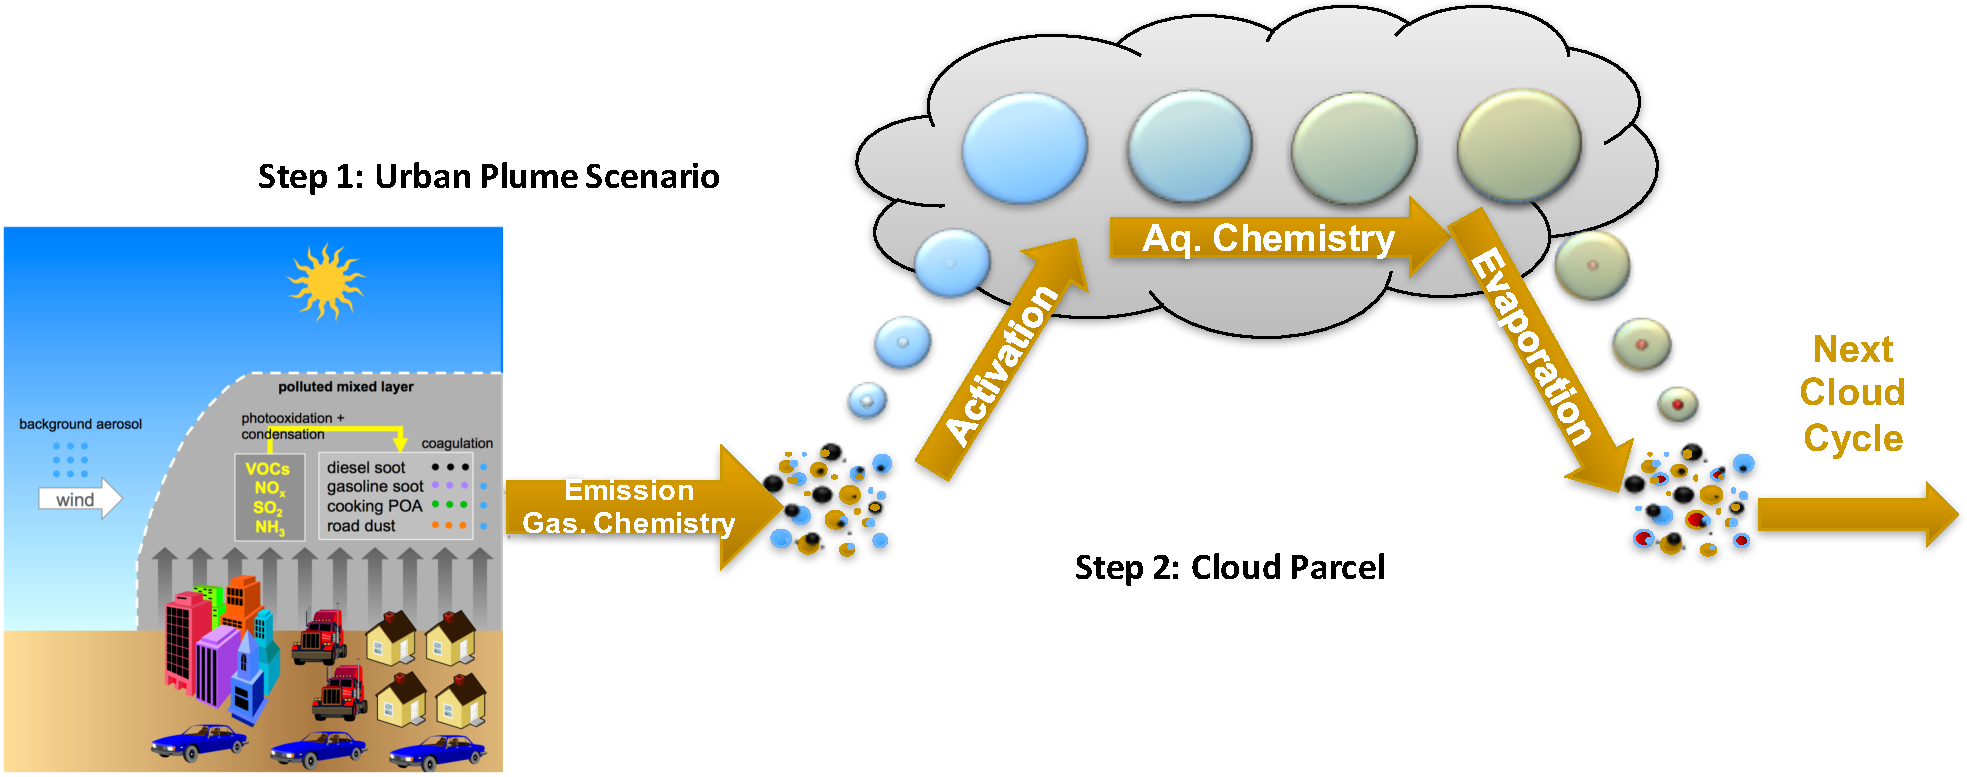
\includegraphics[scale=0.4]{chap2_figs/chap2-fig1-frame.pdf}
    \caption{Two-step cloud chemistry experiment framework}
    \label{chap2-fig1-frame}
\end{figure}

\subsection{Particle-resolved model PartMC-MOSAIC}
PartMC-MOSAIC (Particle Monte Carlo-Model for Simulating Aerosol Interactions and Chemistry) is a Lagrangian box model which simulates the evolution of individual particles by different processes. The evolution is simulated in a well-mixed computational volume and the particle spatial positions are not stored. Compositions of each particle are explicitly tracked by representing the particle as an $A$-dimension vector $\vec{\mu}^i \in \mathbb{R}^A$ with components ($\vec{\mu}_1^i,\vec{\mu}_2^i,...,\vec{\mu}_A^i$), where $\vec{\mu}_a^i$ is the mass of species $a$ in particle $i$, with $a$ = $1,...,A$ and $i$ = $1,...,N$. The evolution for aerosol number concentration with species mass $\mu$ at time $t$, $n(\vec{\mu},t)$, is described by: 
\begin{equation}
\begin{aligned}
 \frac{\partial n(\vec{\mu},t)}{\partial t} &= \underbrace{\frac{1}{2}\int_0^{\mu_1}\int_0^{\mu_2}...\int_0^{\mu_A} K(\vec{\mu}',\vec{\mu}-\vec{\mu}')n(\vec{\mu}',t)n(\vec{u}-\vec{u}',t)d{\mu_1}'d{\mu_2}'...d{\mu_A}'}_\text{coagulation gain}\\
& - \underbrace{\int_0^\infty\int_0^\infty...\int_0^\infty K(\vec{\mu},\vec{\mu}')n(\vec{\mu},t)n(\vec{\mu}',t)d\mu_1'd\mu_2'...d\mu_A' }_\text{coagulation loss} + \underbrace{\dot{n}_{\rm emit}(\vec{\mu},t)}_\text{emission} + \underbrace{\lambda_{\rm dil}(t)(n_{\rm back}(\vec{u},t))-n(\vec{\mu},t)}_\text{dilution}\\
&-\underbrace{\sum_{i=1}^{C}\frac{\partial}{\partial\mu_i}(c_iI_i(\vec{\mu},\vec{g},t))n(\vec{\mu,t})}_\text{gas-particle transfer} - \underbrace{\frac{\partial}{\partial\mu_{C+1}}(c_wI_w)(\vec{\mu},\vec{g},t))n(\vec{\mu,t})}_\text{water transfer} + \underbrace{\frac{1}{\rho_{\rm dry}(t)}\frac{d\rho_{\rm dry}(t)}{dt}n(\vec{\mu},t)}_\text{air density change},
\end{aligned}
\label{eq:partmc}
\end{equation}
where $K$ is the coagulation rate between the particles, $\dot{n}_{\rm emit}(\vec{\mu},t)$ is the emitting distribution of species $\vec{\mu}$, $\lambda_{\rm dil}$ is the dilution rate with background species concentration $n_{\rm back}$, $c_i$ is the gas to particle conversion rate, $I_i$ is the gas species condensation flux, $c_{\rm w}$ is the gas to water conversion rate and $I_{\rm w}$ is the water condensation flux. More details of the equation can refer to \citet{Riemer2009}.

The evolution processes involved in the equation~\ref{eq:partmc} alter the aerosol population in two mechanisms. By adding or removing particles from the population, emission, dilution and coagulation processes modify the number concentration of the population and these processes are accomplished by PartMC with a stochastic Monte Carlo approach. While on the other hand, composition of each particle can be altered by species condensation and evaporation, which are explicitly simulated by state-of-art aerosol chemistry module MOSAIC. In MOSAIC, gas phase reactions are accomplished by carbon bond mechanism CBM-Z, 77~species and 142~reactions are included \citep{Zaveri1999}. Key aerosol species are treated, including $\rm SO_4^{2-}$, $\rm NO_3^-$, $\rm NH_4^+$, BC, primary organic aerosol (POA) and Secondary organic aerosol (SOA). Activity coefficients of electrolytes and ions in aqueous solutions are estimated by multicomponent Taylor expansion method (MTEM), and intraparticle solid-liquid partitioning are treated by Multicomponent Equilibrium Solver for Aerosols (MESA) \citep{zaveri2005computationally}.

PartMC-MOSAIC had been applied to analyze the particle evolution at different environment. For example, \citet{Zaveri2010a} found particle absorption ability increased by 40\% during a 48-hour idealized urban plume condition due to the aging of BC-contained particles. \citet{tian2014modeling} used the model to investigate the processes responsible for the particle number concentration change in a ship plume environment and evaluated the effects of different aging process on particle CCN properties. PartMC-MOSAIC was also used as a benchmark model to quantify the errors in aerosol optical and microphysical properties introduced by simplified mixing state assumptions commonly used in other aerosol models \citep{Zaveri2010a, ching2012impacts, Fierce2017}. PartMC-MOSAIC was further coupled with a cloud parcel model to investigate the effects of mixing state on cloud droplet properties \citep{ching2012impacts, Ching2016}, and the cloud parcel model will be discussed in detail in section~\ref{section:cloud-parcel-model} because this model was also applied for the research both in  this chapter and chapter~\ref{chapter3}. 

\subsection{Cloud parcel model}
\label{section:cloud-parcel-model}
The cloud parcel model coupled with PartMC-MOSAIC is an zero-dimensional adiabatic model. It simulates the particle activation and condensation growth in a rising air parcel and tracks the changes of environment saturation due to the growth of particles and temperature change. Specifically, for a population with $N$ particles of diameter $D_i$, both the growth rate of $D_i$ and the change of environment saturation $S_v$ are diagnosed, which sums to $N$ + 1 state variables to be numerically solved by the model. To focus on the effects of chemical compositions on cloud droplets formation, entrainment, surface tension effects on droplets growth are not included in the model. This section briefly introduces the main equations solved by the parcel model. See \citet{ching2012impacts} for more detailed description of the model. 

During the condensational growth process, the chemical compositions of particle are assumed to be constant and only the water content of the particle alters. The growth rate of particle $i$ is calculated as
\begin{equation}
\centering
\frac{dD_i}{dt} = \frac{G}{D_i}(S_{\rm v}-S_{\rm eq})
\label{eq:cloud-parcel} 
\end{equation}
where the growth coefficient $G$ and droplet equilibrium supersaturation $S_{\rm eq}$ are
\begin{equation}
\centering
\begin{aligned}
 G & = \frac{4D'_{v,i}M_{\rm w}P^0}{\rho_{\rm w}RT}  ,\\
 S_{\rm eq} & = \frac{a_{{\rm w},i}}{1+\delta_i}{\rm exp}(\frac{4M_{\rm w}\sigma_{\rm w}}{\rho_{\rm w}RTD_i}\frac{1}{1+\delta_i} + \frac{\Delta H_{\rm v}M_{\rm w}}{RT}\frac{\delta_i}{1+\delta_i}),
\end{aligned}
\end{equation}
and $D'_{v,i}$ is the modified particle diffusivity, $M_{\rm w}$ and $\rho_{\rm w }$ are the water molecular weight and density, $P^0$ is the saturation vapor pressure, $R$ is the gas constant, $T$ is the environment temperature, $a_{w,i}$ is the water activity of the particle, $\sigma_{\rm w}$ is the water surface tension, $\Delta H_{\rm v}$ is latent heat of vaporization, and $\delta_i$ is defined as 
$$\delta_i = \frac{\Delta H_{\rm }\rho_{\rm w}}{4k'_{{\rm a},i}T}D_i\frac{dD_i}{dt},$$
where $k'_{{\rm a},i}$ is the corrected air thermal conductivity. 

The water activity is calculated by using the parameter $\kappa$ derived by \citet{Petters2007} and can be expressed as
\begin{equation}
\centering
a_{{\rm w},i} = \frac{v_i^{\rm w}}{v_i^{\rm w} + \kappa_i v_i^{\rm dry}},
\label{eq:activity coeff}    
\end{equation}
where $v_i^{\rm w}$ and $v_i^{\rm dry}$ are the volume of water and all the other dry components in particle $i$, respectively. $\kappa_i$ is volume-weighted $\kappa$ of the non-water species. In current model, we used $\kappa$ of 0.65 for ammonium-sulfate-nitrate system, SOA with $\kappa$ = 0.1 and POA with $\kappa$ = 0.001. BC is assumed to be hyrophobic and has $\kappa$ of 0. 

Rather than describing the rising parcel using a constant updraft velocity \citep{Seinfeld2016,rothenberg2016metamodeling}, this parcel model prescribed a constant temperature lapse rate, following the strategy used in \citet{majeed2001microphysics}, to avoid dealing with radiative heating effects. Pressure is also assumed to be constant. In light of these considerations, the change of environment saturation can be given by
\begin{equation}
    \centering
    \frac{dS_{\rm v}}{dt} = -\sum_{i=1}^{N}\frac{\pi \rho_{\rm w} RT}{2M_{\rm w}P^0V_{\rm comp}}D_i^2\frac{dD_i}{dt} - \frac{1}{P^0}\frac{\partial P^0}{\partial T}S_{\rm v}\frac{dT}{dt}
\end{equation}
where the first term describes the effects due to the radius change of all $N$ particles and the second term is about the temperature change. $V_{\rm comp}$ is the computational volume. 

%The coupled model had been used to evaluate the relative importance of particle size and compositions for cloud droplet concentration. 

\subsection{Aqueous chemistry model}
\label{section:aq-chem-model}
In this work, PartMC-MOSAIC was further coupled with an aqueous chemistry module based reduced Chemical Aqueous Phase Radical Mechanism(CAPRAM) version 2.4. The full mechanism in CAPRAM 2.4 includes 439 reactions and 147 species, and a reduced version is also provided to be more computationally efficient, which includes 183 reactions and 113 species \citep{Ervens2003}. The reduced version also contains a comprehensive aqueous mechanism, and deals with the reactions between OH, $\rm HO_2$, $\rm NO_3$, $\rm SO_4$, $\rm Cl_2$,$\rm Br_2$ and $\rm CO_3$ with inorganic (TMIs, $\rm NO_3^-$ , $\rm Cl^-$, $\rm Br^-$) and organic reactants with less than two atoms. The constants for thermodynamic and kinetic reactions are listed in Table~\ref{tab:capram}. When coupling CAPRAM with PartMC-MOSAIC, the original gas phase chemistry mechanism, Regional Atmospheric Chemistry Modeling (RACM), used in CAPRAM 2.4 is now replaced with CBM-Z in PartMC-MOSAIC. 

\subsection{Ensemble monodisperse simualtion settings}
This work is the first application of particle-resolved cloud chemistry model, and we used relative simple aerosol description, that is the monodisperse distribution, to investigate aqueous sulfate processes. More complex populations with lognormal distribution and the role of other cloud processes, such as coagulation between interstitial particles and cloud droplets, are explored in next chapter. 

We created a scenario ensemble by exposing the monodisperse aerosol populations at different chemical and physical environment, denoted as
$P_{\rm ref}$. We set the initial particle size at 100 \unit{nm} composed of ammonium sulfate. Emission and dilution are also not included in current simulations. Four important gas species for aqueous sulfate formation, including $\rm O_3$, $\rm H_2O_2$, $\rm NH_3$ and $\rm SO_2$, are perturbed at low, medium and high polluted levels, as listed in table~\ref{TMI-setting}. The $\rm O_3$ and $\rm SO_2$ values of these three levels are based on the national wide urban measurements in China \citep{wang2014spatial}, and $\rm NH_3$ levels are determined from the observations of Houston, U.S. \citep{nowak2010airborne} and Seoul, Korea \citep{phan2013analysis}. The values for $\rm H_2O_2$ are based on the measurements in Guangzhou, China \citep{hua2008atmospheric}. We also set three different temperature rates to provide cloud environment with varied liquid water content, and the corresponded cloud updraft velocity are 1.1, 1.5 and 1.8\unit{m\;s^{-1}} respectively, which represent the conditions of strong convective stratus \citep{peng2005importance}. In total, we simulated $3^5$ = 243 cases in this ensemble scenario.

\begin{table}[ht]
\centering
\caption{Settings for monodisperse simulation}
\label{TMI-setting}
\begin{tabular}{c  c c  c}
\hline
Parameters & Low  & Medium & High\\
\hline
$\rm O_3$& 25 & 50 & 75 \\
$\rm H_2O_2$& 0.25 & 0.5 &  1\\
$\rm NH_3$ &2 & 4 & 6 \\
$\rm SO_2$&2&5& 10\\
$\rm \frac{dT}{dt}$ &$-$0.3 &$ -$0.4&$-$0.5\\
\hline
\end{tabular}
\end{table}

The initial RH is 99\% and the simulation last 20 minutes. As showed in Fig.~\ref{chap2:ensemrh}, cases with higher temperature lapse rates experience more rapid increase of liquid water content, while the reached maximum supersaturation are close between the cases. Cloud formed in the first minute and the maximum supersaturation is 0.2\%. 

\begin{figure}[ht]
    \centering 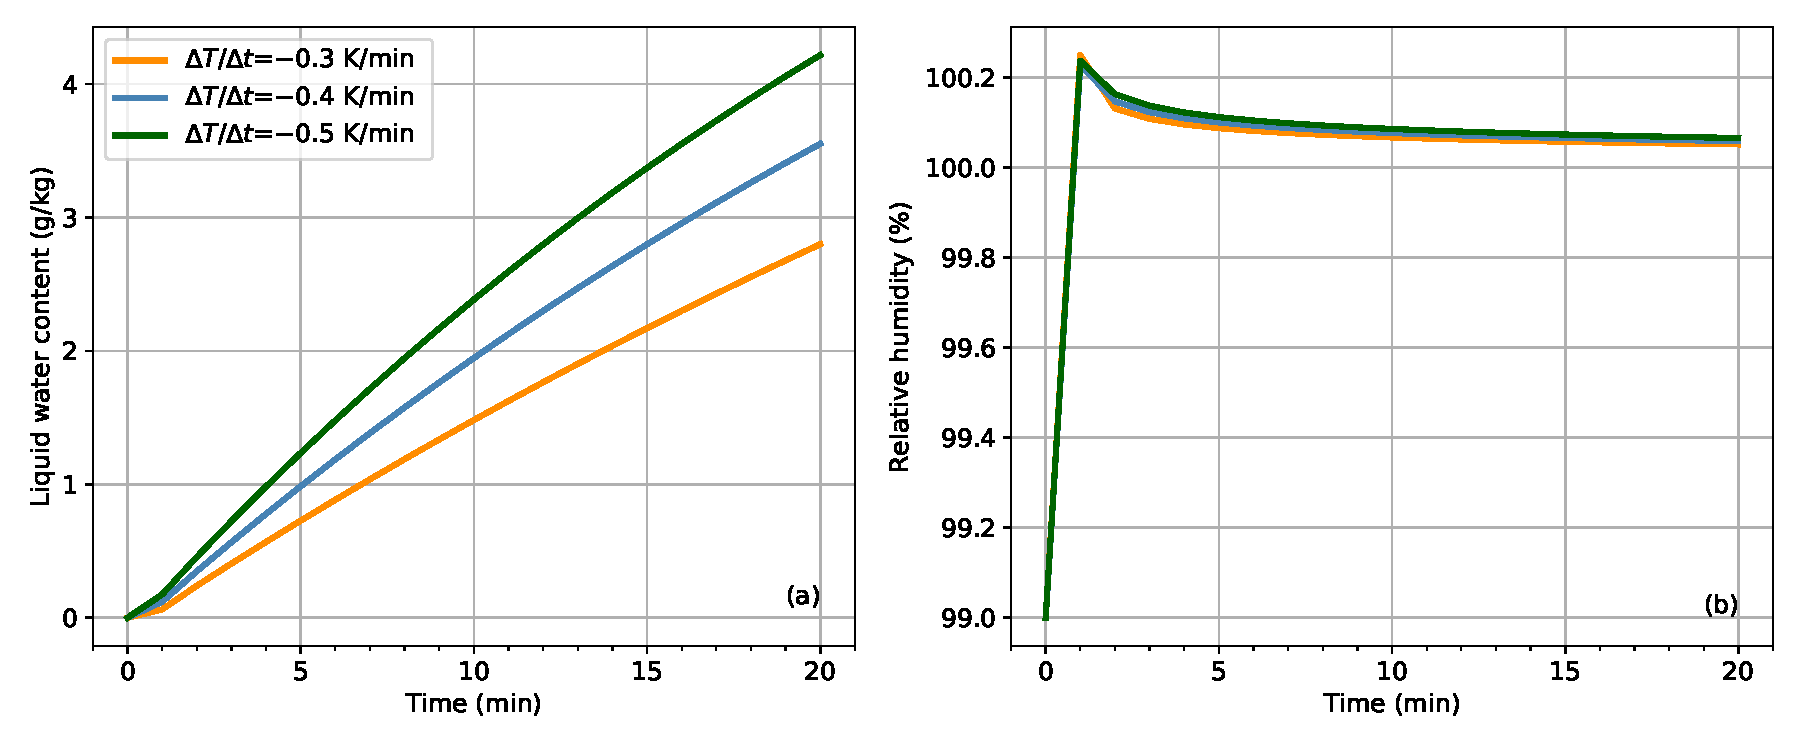
\includegraphics[scale=0.6]{chap2_figs/chap2_mono_lwc_rh.pdf}
    \caption{Time series of (a) liquid waeter content and (b) relative humidity in the ensemble scenarios. Blue, orange and green lines are for the cases with temperature lapse rate of --0.3 \unit{K/min}, --0.4 \unit{K/min} and --0.5 \unit{K/min} respectively.}
    \label{chap2:ensemrh}
\end{figure}

In order to figure out the role of TMI pathways for aqueous sulfate formation, we created another scenario ensemble, denoted as $P_{\rm TMI}$ by adding $\rm Fe(II)$ and $\rm Fe(III)$ in the initial aerosol population. We set the mass fraction of $\rm Fe(II)$ and $\rm Fe(III)$ to be 0.05 and 0.01. \citet{deguillaume2004role} found aqueous hydroxide is important for TMI oxidation pathways and the concentration is in the order of $\rm 10^{-13}$~\unit{M}. We achieved this  by emitting gas OH at the rate of $2\times 10^{-8}$ \unit{mole/m^2/s}. We also applied the same perturbed parameters as in $P_{\rm sul}$, which results in another 243 cases for $P_{\rm TMI}$. 

\section{Sulfate mechanism verification}
Before applying the comprehensive particle-resolved aqueous chemistry model to study the role of different aqueous sulfate pathways, we first evaluated it by comparing with the models used in \cite{kreidenweis2003modification}(hereafter, KS2003). In KS2003, several bulk and size-resolved models were used to simulate aqueous sulfate formation in an adiabatic updraft cloud environment. They found significant differences in $\rm SO_2$ oxidation rates between size-resolved and bulk models. This model comparison work provides a benchmark for checking aqueous sulfate mechanisms, and we used the same simulation setting in that work to verify our particle-resolved aqueous chemistry approach. Physical and chemical conditions, including the updraft velocity, temperature change, initial species concentration and chemical equations are all set to the same with values used in KS2003, as listed in table~\ref{setting}. In the models used in KS2003, cloud formed by a constant updraft velocity. But in our model, as mentioned before, we predefined the temperature lapse rate. In order to get the same updraft velocity, we obtained the temperature values of constant updraft velocity at 0.5 from pyrcel model, a zero-dimensional adiabatic cloud parcel model \citep{rothenberg2016metamodeling}. 

\begin{table}[ht]
\centering
\begin{threeparttable}
\caption{Cloud  chemical and physical conditions}
 \begin{tabular}{l c|c l}
 \hline
  Physical arameters & Value (Units) & Chemical parameters ($t = 0$) & Values Units\\
 \hline
 Temperature at $t =0$ & 285.2 (K)&$\rm SO_2$ & 200 (pptv)\\
 Pressure at t = 0 & 950 (mbar)&$\rm NH_3$ & 100 (pptv)\\
 Updraft velocity & 0.5 ($\rm m\,s^{-1}$)&$\rm H_2O_2$ & 500 (pptv)\\
 Cloud water mixing ratio after 2400 s& 2.17 ($\rm g\,kg^{-1}$)&$\rm HNO_3$  & 100 (pptv)\\
 Air density at the cloud base & 1.15 ($\rm kg\,m^{-3}$) & $\rm O_3$ &50 (ppbv)\\
 Cloud base temperature& 284.2 K&$\rm CO_2$ & 360 (ppmv)\\
 Cloud base pressure& 939 (mbar)& $\rm SO_4^{2-}$ & 2 ($\rm \mu g \, m^{-3}$)\\ 
 Relative humidity at t =0 & 95$\rm \%$ & $\rm NH_4^+$ & 0.375 ($\rm \mu g\, m^{-3}$)\\
 \hline
 \label{setting}
\end{tabular}
\end{threeparttable}
\end{table}

Figure~\ref{chap2:ks2003}(a) shows the simulated cloud liquid water content (LWC). PartMC simulated higher LWC changing rate and it is it may result from the different cloud parcel model settings. As mentioned before, we prescribed a constant temperature lapse rate. But for models used in KS2003, a constant updraft velocity is described. Another possible factor is the treatment of droplet surface temperature $T$, which is used to calculate droplet growth rate and it is common for models to assume $T$ equals to environment temperature $T_\infty$. But in our model, we did not use this assumption and the different treatments may also result in the calculated LWC differences.

\begin{figure}[ht]
    \centering 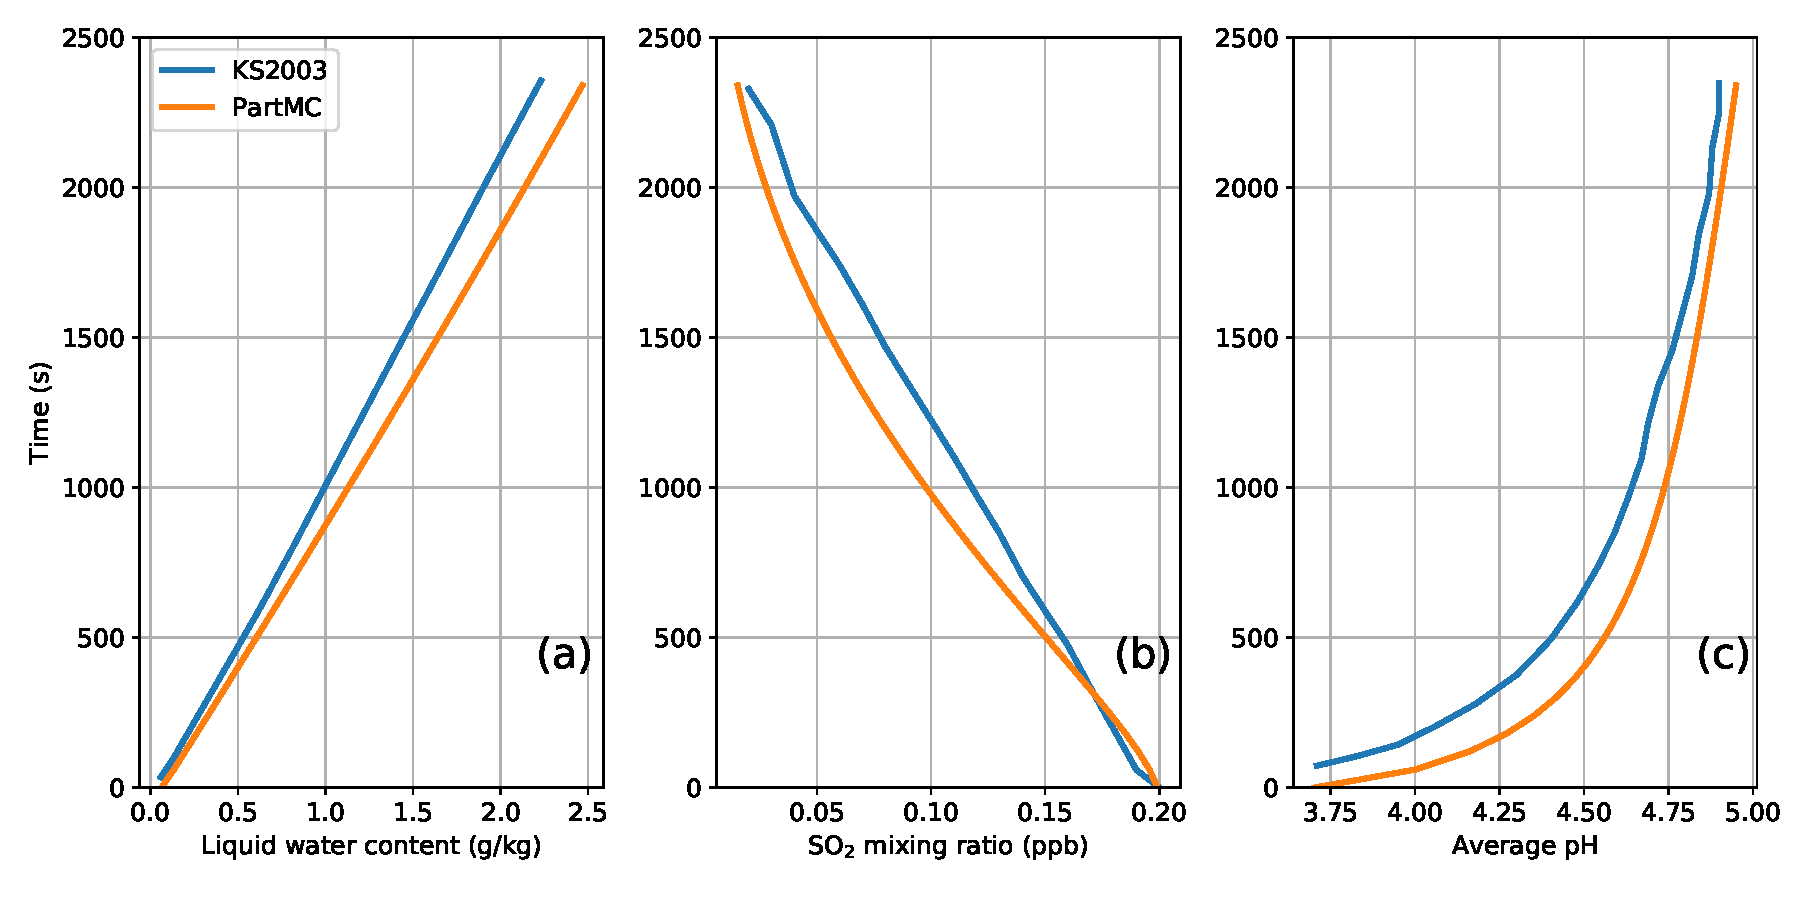
\includegraphics[scale=0.5]{chap2_figs/chap2_fig1_profile.pdf}
    \caption{Vertical profile differences of (a) liquid water content and (b) Gas $\rm SO_2$ concentration (c) Bulk pH between KS2003 and PartMC.}
    \label{chap2:ks2003}
\end{figure}

The simulated $\rm SO_2$ depleting rate is almost consistent between PartMC and KS2003 (Fig.~\ref{chap2:ks2003}(b)), with $\rm SO_2$ gas mixing ratio decreasing from 0.2 to 0.025~ppb after 40 minutes, indicating PartMC is capable of simulating of aqueous sulfate formation processes. The bulk acidity calculated by PartMC also shows similar profile with the models in KS2003 but with higher values (Fig.~\ref{chap2:ks2003}(c)). Considering the different simulation approaches, we are expecting the differences between bulk or size-binned based pH and our particle-resolved pH. 

Since sulfate aqueous formation pathways are highly acidity dependent, especially through $O_3$, where reaction rates increase exponentially with increasing pH, the acidity differences imply noticeable changes in sulfate production. At the end of simulation, PartMC simulated sulfate concentration of 207 ppb, higher than the $\sim$ 175 in size-resolved models and $\sim$ 145 in bulk models. As explained in KS2003, the excess produced sulfate in the size-resolved models are found to be associated with higher simulated pH and more sulfate formed from $O_3$ oxidation pathway. This explanation is still applicable for our current findings. 

In summary, this comparison simulation proved our particle-resolved aqueous model is capable of capturing the sulfate aqueous chemical processes. 
With more detail particle information, our particle-resolved approach may also provide more comprehensive understanding of different sulfate formation pathways, and this is explored in our next section. 
%\begin{figure}
\section{Contribution of different aqueous formation pathway}

This section explored the important factors for higher aqueous sulfate formation by analyzing the 243 aerosol populations in $P_{\rm ref}$.
Figure~\ref{chap2:ens_three} shows the different sulfate formation rates in the ensemble scenarios. We found there are clear sulfate formation separations between the cases with different ammonia gas mixing ratio and cases with more sulfate production are associated with high ammonia environment. But this separation is not clear for other two considered factors, because cases with higher sulfate formation can be with all the three levels of temperature lapse rate and $\rm H_2O_2$ gas mixing ratio. This phenomena indicates ammonia gas concentration is a determined factor for aqueous sulfate formation in current simulated scenarios. The role of other factors are further explored in Fig.~\ref{chap2:factor}.

\begin{figure}[ht]
    \centering 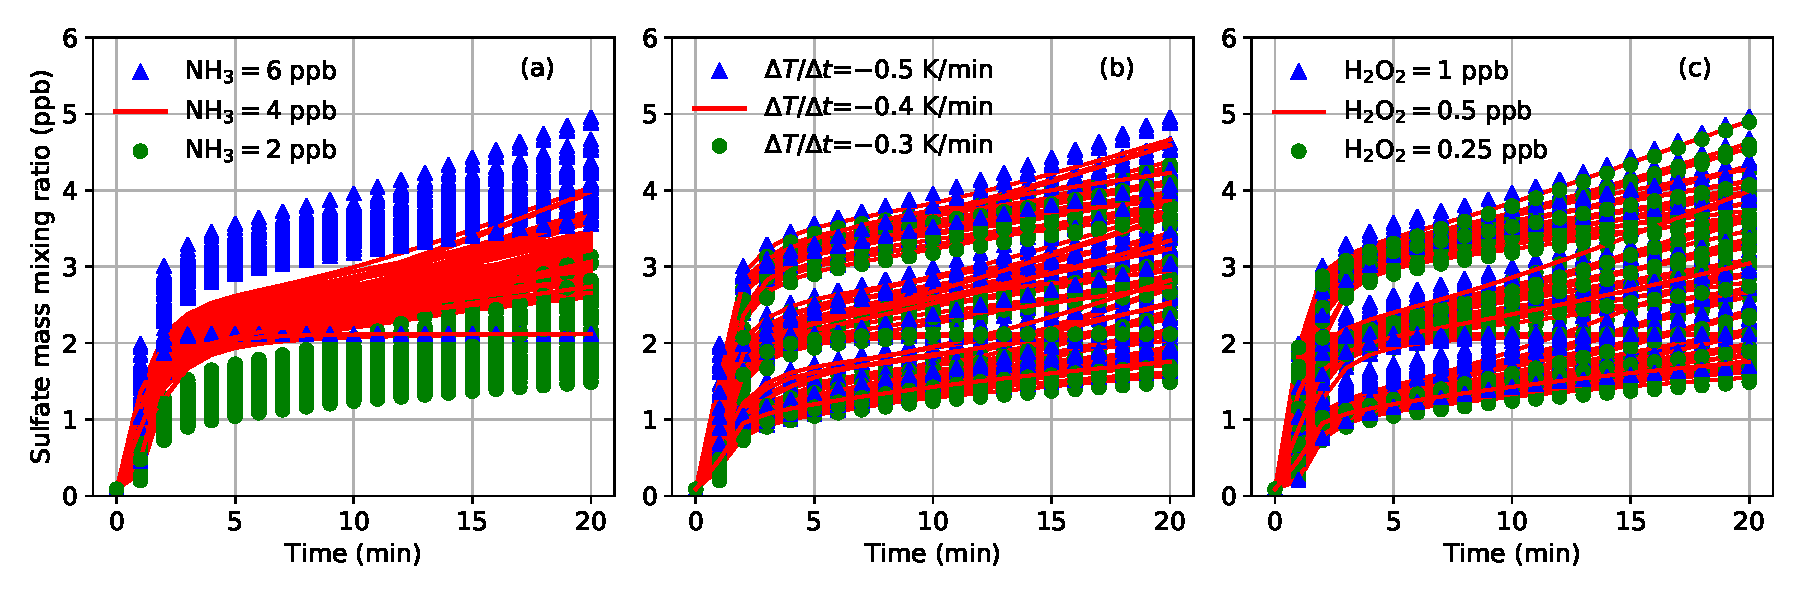
\includegraphics[scale=0.6]{chap2_figs/chap2_fig2_mono_ensemble.pdf}
    \caption{Sulfate time series categorized by three different settings in $P_{\rm ref}$: (a) initial ammonia gas mixing ratio (b) temperature lapse rate (c) initial $\rm H_2O_2$ gas mixing ratio. The three colors and symbols are for the low, medium and high levels of each parameter.}
    \label{chap2:ens_three}
\end{figure}

Figure~\ref{chap2:factor} shows the connection between sulfate concentration at 20~\unit{min} and the environment settings. All the cases with sulfate concentration over 4~\unit{ppb} are associated with $\rm NH_3$ of 6~\unit{ppb}. There is no clear relation between the high sulfate values and $\rm O_3$ and $\rm H_2O_2$ mixing ratio since high sulfate production cases are evenly distributed in all the levels. We also found $\rm SO_2$ level is neither a good indicator for high sulfate formation. 

\begin{figure}[ht]
    \centering 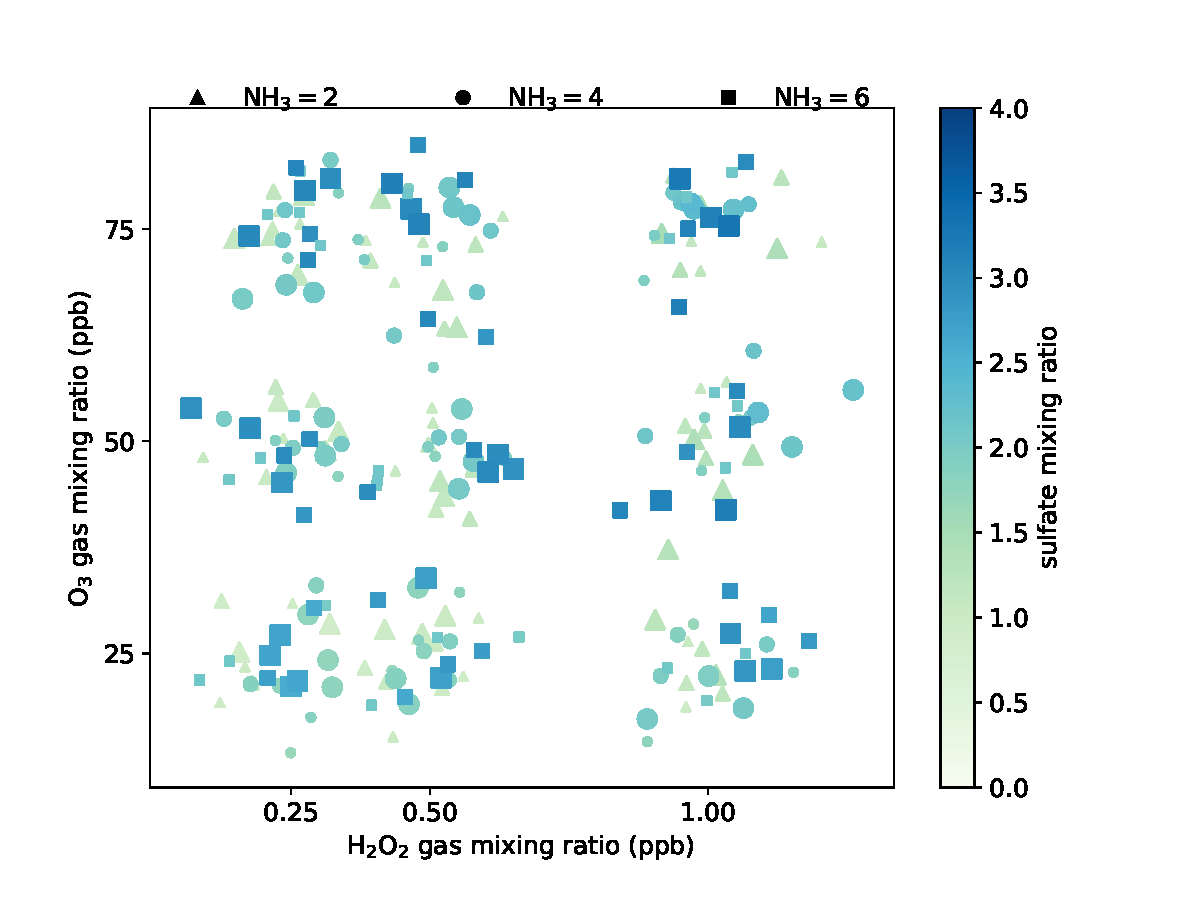
\includegraphics[scale=0.7]{chap2_figs/chap2_fig3_sulfate_scatter.pdf}
    \caption{Relation between sulfate concentration at 20~\unit{min} and the parameters in $P_{\rm ref}$. Color represents the sulfate concentration. Triangle, circle and square are for case with 2~\unit{ppb},  4~\unit{ppb} and 6~\unit{ppb} $\rm NH_3$ respectively. Marker size indicates $\rm SO_2$ level.}
    \label{chap2:factor}
\end{figure}

Figure~\ref{chap2:su-acidity} shows the relation between sulfate mixing ratio and particle acidity at 3~\unit{min}. At the same $\rm SO_2$ level, cases with higher $\rm NH_3$ produced more sulfate. The increasing rate is higher for higher $\rm SO_2$ cases, average sulfate mixing ratio increased from 1.1 ppb to 3.0 ppb at with $\rm SO_2$ of 10~\unit{ppb}, while the change is only 1~\unit{ppb} in the cases with 2~\unit{ppb} $\rm SO_2$. This indicates at the same $\rm NH_3$ level, sulfate formation is $\rm SO_2$ limited. 

\begin{figure}[ht]
    \centering 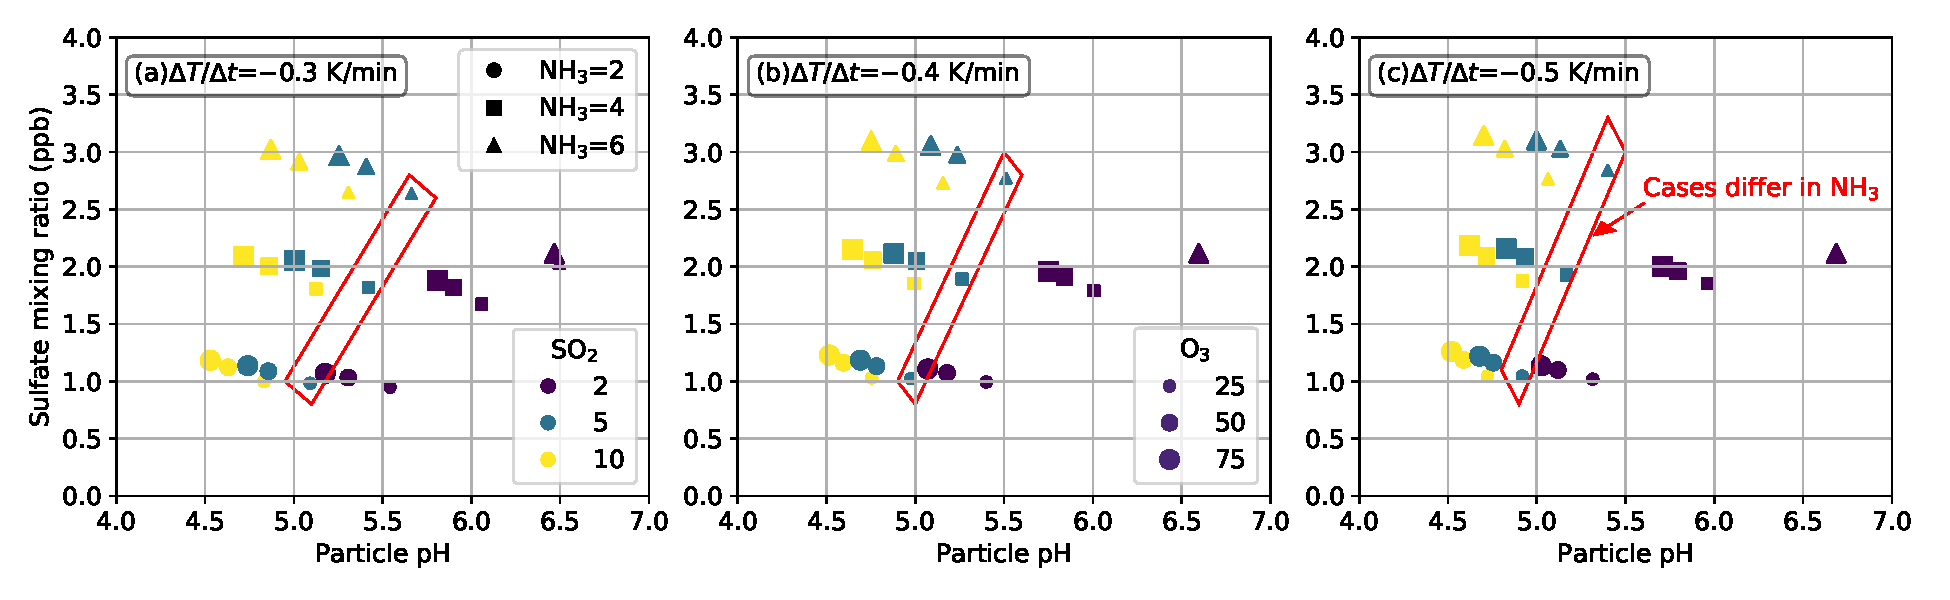
\includegraphics[scale=0.6]{chap2_figs/chap2_fig4_sulfate_pH_3min.pdf}
    \caption{Correlation between sulfate mixing ratio and acidity at 3~\unit{min}. Symbols are colored by $\rm SO_2$ levels. Symbol types are for $\rm NH_3$ levels.}
    \label{chap2:su-acidity}
\end{figure}

Reaction rates of three main aqueous sulfate formation pathways are explored in Fig.~\ref{chap2:reac-rates}. Sulfate formation through $\rm H_2O_2+ HSO_3^-$ and $\rm O_3+ SO_3^{2-}$ pathways are 1--2 orders higher than $\rm O_3 + HSO_3^-$. The oxidation rates of $\rm HSO_3^-$ by $\rm H_2O_2$ and $\rm O_3$ increase rapidly with increasing $\rm SO_2$ gas mixing ratio. For the cases with 6~\unit{ppb} $\rm NH_3$, median reaction rates of $\rm H_2O_2+ HSO_3^-$ at jump from $10^{-9}$~\unit{M/s} at 2~\unit{ppb} $\rm SO_2$ to $10^{-7}$~\unit{M/s} at 10~\unit{ppb} $\rm SO_2$. But for oxidation of $\rm SO_3^{2-}$ by $\rm O_3$, the reaction rate and $\rm SO_2$ mixing ratio is negative correlated. That can explain why there is no strong correlation between $\rm SO_2$ mixing ratio and high sulfate formation rates. As for $\rm NH_3$, oxidation rates of $\rm HSO_3^-$ and $\rm SO_3^{2-}$ by $\rm O_3$ is higher at the cases with 6~\unit{ppb} $\rm NH_3$, and there is no clear change for $\rm H_2O_2+ HSO_3^-$ at different $\rm NH_3$ levels. This is consistent with what we found the most sulfate formation cases are connected with high $\rm NH_3$ cases. The only anomalous cases are for the aerosol populations with 2~\unit{ppb} $\rm NH_3$, where the reaction rates decreased with increasing $\rm NH_3$. This is the $\rm SO_2$-limited cases we mentioned above. 

Based on analysis for the cases in $P_{\rm ref}$, we found the aqueous sulfate formation are most sensitive to the $\rm SO_2$ and $\rm NH_3$ mixing ratios. Cases with most sulfate formation are for the cases with high $\rm NH_3$ values and this can be explained by the higher oxidation rates of $\rm SO_3^{2-}$ by $\rm O_3$. Cases with higher $\rm NH_3$ but lower sulfate production are because of lower $\rm SO_2$. Thus, sulfate formation is $\rm SO_2$-limited. 

\begin{figure}[ht]
    \centering 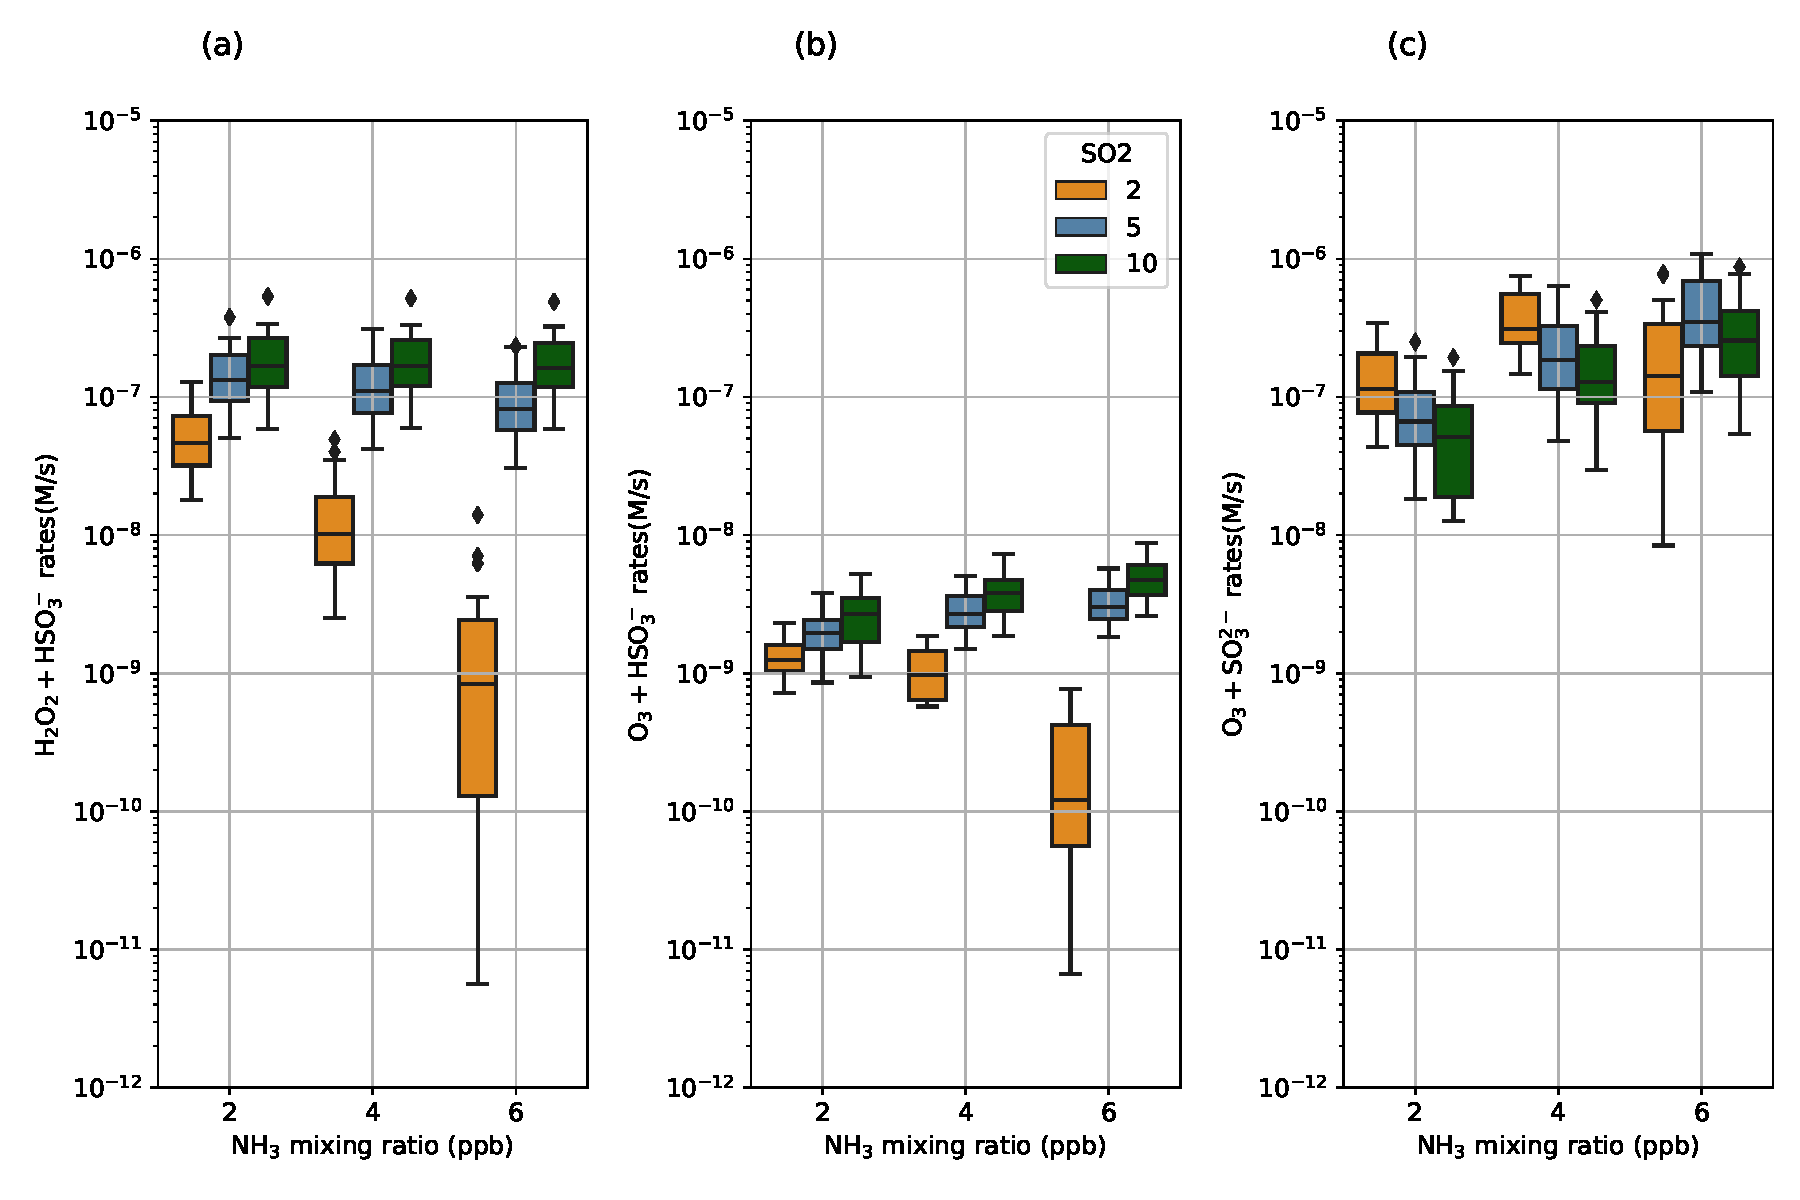
\includegraphics[scale=0.55]{chap2_figs/chap2_fig5_sulfate_rates_3min.pdf}
    \caption{Statistics of three aqueous sulfate formation pathway rates: (a) $\rm H_2O_2+ HSO_3^-$ (b) $\rm O_3+ HSO_3^-$ (c) $\rm O_3+ SO_3^{2-}$. Cases are grouped by $\rm NH_3$ and $\rm SO_2$ mixing ratio.}
    \label{chap2:reac-rates}
\end{figure}

\section{Contribution of TMI pathways}

In this section, we will analyze the other 243 cases containing iron components in $P_{\rm TMI}$. Figure~\ref{chap2:iron-conc}(a) shows the time series of $\rm Fe^{2+}$, $\rm Fe^{3+}$ and OH(aq) mass concentration in the ensemble cases. $\rm Fe^{2+}$ varies between $10^{-11}$ and $10^{-7}$ and $\rm Fe^{3+}$ ranges between $10^{-7}$ and $10^{-6}$~\unit{M}, both are in the same order with the values in \citep{Deguillaume2005}. By adding TMI, the median sulfate mixing ratio in $P_{\rm TMI}$ significantly increased from 2~\unit{ppb} to 5~\unit{ppb}. Figure~\ref{chap2:iron-contri} further explores the contribution ratio changes of different aqueous sulfate pathways after adding TMI in the population. 

\begin{figure}[ht]
    \centering 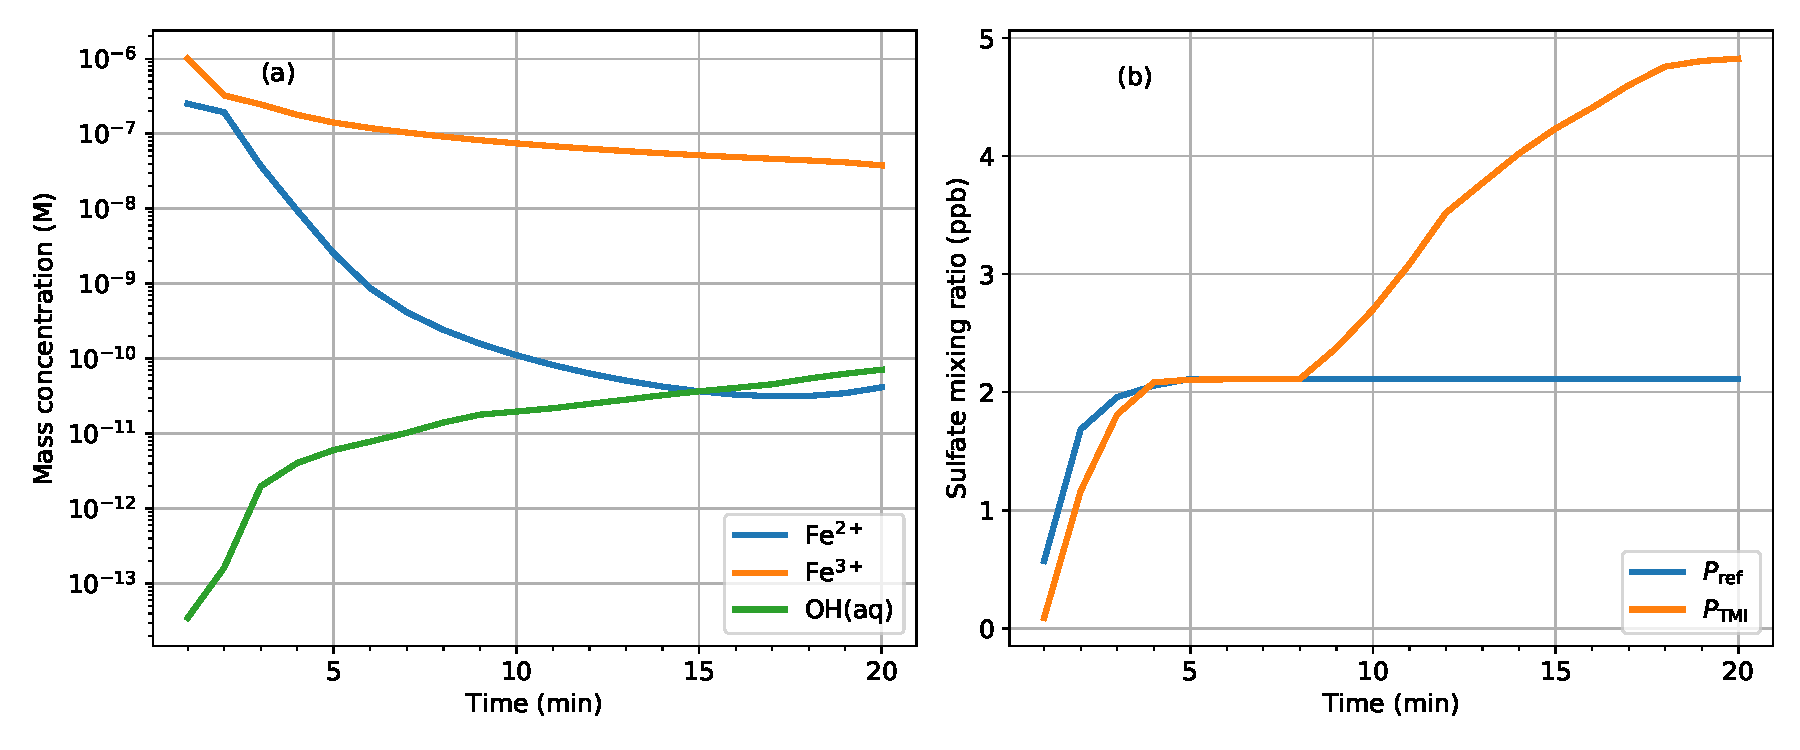
\includegraphics[scale=0.7]{chap2_figs/chap2_with_tmi_fixOH_mass.pdf}
    \caption{Time series of (a) $\rm Fe^{2+}$, $\rm Fe^{3+}$ and $\rm OH(aq)$ (b) Sulfate mixing ratio in $P_{\rm ref}$ and $P_{\rm TMI}$. Values are the median of all the ensemble cases in $P_{\rm TMI}$. }
    \label{chap2:iron-conc}
\end{figure}

Oxidation of $\rm HSO_3^-$ by $\rm O_3$ and $\rm H_2O_2$ are the dominant pathways for aqueous sulfate formation in $P_{\rm ref}$ (Fig.~\ref{chap2:iron-contri}(a)). These two pathways in total contributed to more than 90\% of sulfate formation along the simulation period, and there is minimum contribution of TMI pathways. But in $P_{\rm TMI}$, these two pathways are dominant at the first 2 minutes and sulfate formation through the reaction between $\rm SO_4^-$ and water is dominant afterwards (Fig.~\ref{chap2:iron-contri}(b)). We also noticed a remarkable contribution from TMI pathway after 4~\unit{min}, and the contribution ratio can be more than 20\% at the end of simulation. 

\begin{figure}[ht]
    \centering 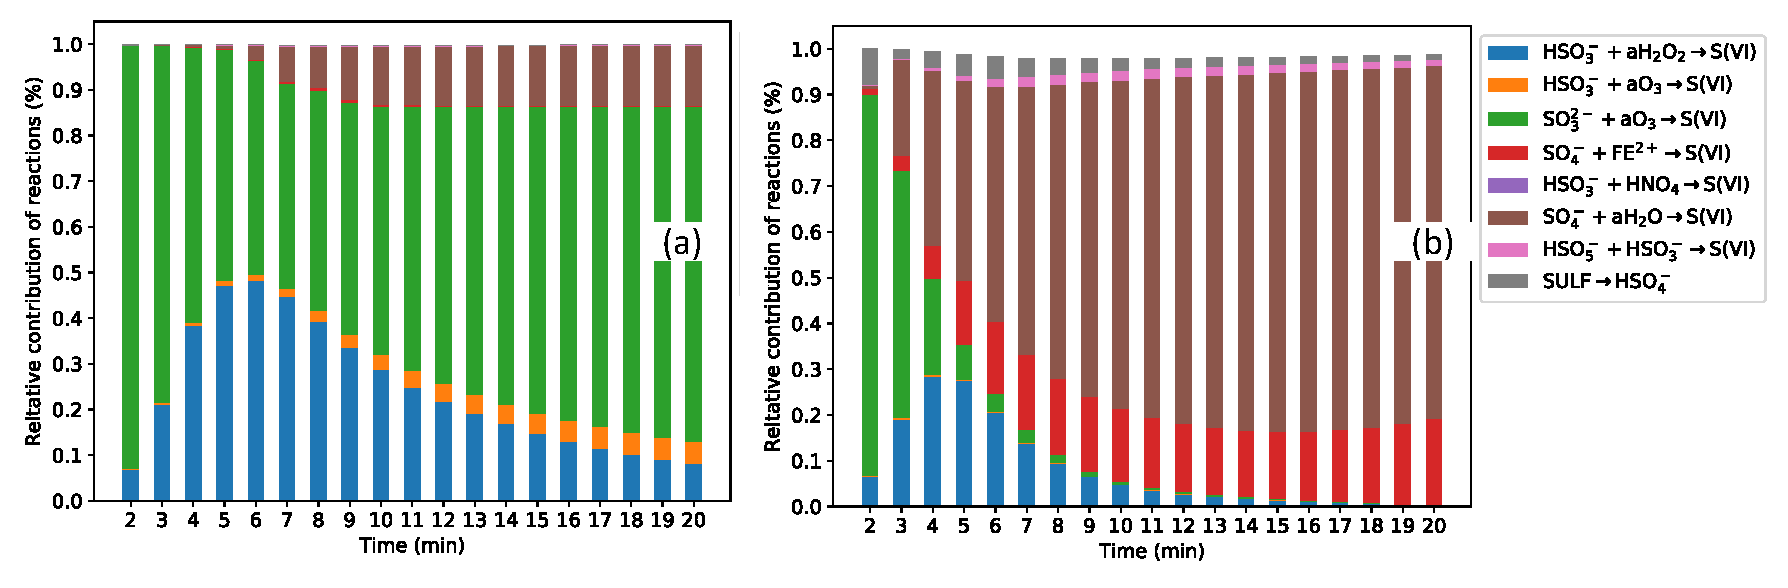
\includegraphics[scale=0.7]{chap2_figs/chap2-TMI_contri_factors.pdf}
    \caption{Mean contribution fraction of different sulfate formation pathways in (a)$P_{\rm ref}$ and (b)$P_{\rm TMI}$}
    \label{chap2:iron-contri}
\end{figure}

It is worth mention that gas OH emitted at a constant rate for the cases $P_{\rm TMI}$, while there is no emission in $P_{\rm ref}$. Based on current simulation setting, we can not distinguish the role of OH and TMI for the increased sulfate production rates in $P_{\rm TMI}$. Further simulations are needed to validate the current findings. But what we can still learn from current result is there exists some conditions where sulfate formation through TMI pathways can be important. 

\section{Conclusion}


\backmatter
\renewcommand{\bibname}{References}
\bibliographystyle{copernicus}
\bibliography{thesis_ref}
\end{document}

\appendix
% Reset the algorithm counter
\setcounter{algorithm}{0}

\chapter{Appendix to Chapter~\ref{chap2:mon}}
\label{tab:capram}
\section{List of aqueous reactions coupled to PartMC-MOSAIC}
This appendix shows the thermodynamic and kinetic data for the aqueous chemistry reactions 
coupled with PartMC-MOSAIC. It is based on the reduced CAPRAM 2.4 mechanism, 
and the full mecahnism can refer to \citet{Ervens2003}.
Table~\ref{Henry} lists the coefficients for Henry's Law.
%%%%%%%Table A1%%%%%%%%
\begin{table}[ht]
\centering
\caption{Henry's Law coefficients} \centering
\label{Henry}
\begin{threeparttable}
\begin{tabular}{ c l c c}
\toprule Henry's Law & Equilibrium & $K_{298}$ (M $\rm atm^{-1}$)$^*$& $-\Delta H/R$ (K) \\ 
\midrule
H1  & \ce{CO_2{(\rm g)}  <=> CO_2{(\rm aq)}} & 3.1$\times 10^{-2}$& 2423 \\ 
H2 & \ce{O_3{(\rm g)} <=> O_3{(\rm aq)}} &1.14 $\times 10^{-2}$ & 2300 \\ 
H3  & \ce{HO_2{(\rm g)}  <=> HO_2{(\rm aq)}} & 1.14$\times 10^{-2}$& 2300 \\ 
H4  & \ce{OH{(\rm g)}  <=> OH{(\rm aq)}} & 9$\times 10^{3}$& 0 \\ 
H5  & \ce{H_2O_2{(\rm g)} <=> H_2O_2{(\rm aq)}} &1.02 $\times 10^{5}$ & 6340 \\ 
H6  &\ce{NO_2{(\rm g)} <=> NO_2{(\rm aq)}} &1.2 $\times 10^{-2}$ & 1263\\
H7  &\ce{HONO{(\rm g)} <=> HONO{(\rm aq)}} & 49 & 4880\\
H8  & \ce{HNO_3{(\rm g)} <=> NO_3^- + H^+} &4.62 $\times 10^{6}$& 10500\\
H9  &\ce{NO_3{(\rm g)} <=> NO_3{(\rm aq)}} &6 $\times 10^{-1}$ & 0\\ 
H10  &\ce{N_2O_5{(\rm g)} <=> N_2O_5{(\rm aq)}} &1.4 $\times 10^{0}$ & 0\\ 
H11 & \ce{NH_3{(\rm g)}  <=> NH_3{(\rm aq)}} & 60.7 & 3920 \\ 
H12 & \ce{HCL{(\rm g)}  <=> CL^{-} + H^{+}} & 1.89$\times 10^6$ & 8910 \\ 
H13 & \ce{HCHO{(\rm g)}  <=> HCHO{(\rm aq)}} & 2.5 & 7216 \\ 
H14 & \ce{ORA{1}{(\rm g)}  <=> ORA{1}{(\rm aq)}} & 5.53$\times 10^3$ & 5630 \\ 
H15 &\ce{SO2{(\rm g)}  <=> SO2{(\rm aq)}} & 1.24 & 3247  \\ 
H16 &\ce{OP{1}{(\rm g)}  <=> OP{1}{(\rm aq)}} & 310 & 5607  \\ 
H17 &\ce{ORA{2}{(\rm g)}  <=> ORA{2}{(\rm aq)}} & 5.5$\times 10^3$ & 5890  \\ 
H18 &\ce{MO{2}{(\rm g)}  <=> MO{2}{(\rm aq)}} & 310 & 5607  \\ 
H19 &\ce{ETHPX{(\rm g)}  <=> ETHPX{(\rm aq)}} & 340 & 87  \\ 
H20 &\ce{ETOH{(\rm g)}  <=> ETOH{(\rm aq)}} & 190 & 6290  \\ 
H21 &\ce{CH{3}OH{(\rm g)}  <=> CH{3}OH{(\rm aq)}} & 220 & 5390  \\ 
H22 &\ce{ALD{(\rm g)}  <=> ALD{(\rm aq)}} & 4.8 & 6254  \\ 
H23 &\ce{BR{2}{(\rm g)}  <=> BR{2}{(\rm aq)}} & 0.758 & 3800  \\ 
H24 &\ce{CL{2}{(\rm g)}  <=> CL{2}{(\rm aq)}} & 9.15$\times 10^{-2}$ & 2490  \\ 
H25 &\ce{SULF{(\rm g)}  <=> HSO_4^- + H^{+}} & 8.7$\times10^{11}$ & 0 \\
H26 &\ce{HNO4{(\rm g)}  <=> HNO4{(\rm aq)}} &3$\times 10^4$& 0 \\ 
H27 &\ce{ACO3{(\rm g)}  <=> ACO3{(\rm aq)}} &6.69$\times 10^4$& 5893 \\ 
H28 &\ce{GLY{(\rm g)}  <=> GLY{(\rm aq)}} &1.40& 0 \\ 
H29 &\ce{[O_2]^{**}{(\rm g)}  <=> O_2{(\rm aq)}} &1.3$\times 10^{-3}$& 1700 \\ 
\bottomrule
\end{tabular}
\end{threeparttable}
\end{table}

% Table continued on next page
\addtocounter{table}{-1}
\begin{table}[ht]
\centering
\begin{threeparttable}
\caption{Continued.}
\begin{tabular}{ c l c c}
\toprule Henry's Law & Equilibrium & $K_{298}$ (M $\rm atm^{-1}$) & $-\Delta H/R$ (K) \\ 
\midrule
H30 &\ce{CLNO2{(\rm g)}  <=> CLNO2{(\rm aq)}} &0.024& 0.0 \\ 
H31 &\ce{BRNO2{(\rm g)}  <=> BRNO2{(\rm aq)}} & 0.3 & 0.0 \\ 
H32 &\ce{BRCL{(\rm g)}  <=> BRCL{(\rm aq)}} &0.94& 0.0 \\ 
H33 &\ce{NO{(\rm g)}  <=> NO{(\rm aq)}} &1.9$\times 10^{-3}$& 0.0 \\ 
\bottomrule
%\vspace*{5mm}
\end{tabular}
\begin{tablenotes}[para,flushleft]
      \small
      \item $*$: $K = K_{298} {\rm exp}(-\frac{\Delta H}{R}(\frac{1}{T}- \frac{1}{298}))$\\
      \item $**$: Specie with square bracket indicates its concentration is constant. 
\end{tablenotes}
\end{threeparttable}
\end{table}

Table~\ref{aq-ox} lists the coefficients for aqueous chemical reactions. 
%%%%%%Table A2%%%%%%%%%%%%
\begin{table}[ht]
\centering
\caption{Aqueous chemical reactions} \centering
\label{aq-ox}
\begin{threeparttable}
\begin{tabular}{ c l c c}
\toprule Aqueous chemistry & Reaction & $ K_{298}$ (${\rm M}^{-n}$ $\rm s^{-1}$) & $-E/R$ (K) \\ 
\midrule
A1 & \ce{FEOH^{2+} -> FE^{2+} + OH(\rm aq)} & 4.76$\times 10^{-3}$ & 2.20 \\
A2 & \ce{NO3^{-} -> NO2(\rm aq) + OH(\rm aq) + OH^{-}}& 4.57$\times 10^{-7}$ & 2.59 \\
A3 & \ce{H2O2(\rm aq) -> OH(\rm aq) + OH(\rm aq)} & 7.64$\times 10^{6}$ & 2.46 \\
A4 & \ce{FEC2(O4)_2^{-} -> FE^{2+} + C2O4^{2-} + CO2(\rm aq) + CO2^{-}} &2.47 $\times 10^{-2}$& 1.96 \\
A5 & \ce{H2O2(\rm aq) + FE^{2+} -> FE^{3+} + OH(\rm aq) + OH^{-}} & 50.0 & 0.0 \\
A6 & \ce{H2O2(\rm aq) + Cu^+ -> Cu^{2+} + OH(\rm aq) + OH^-} & 7000.0 & 0.0 \\
A7 & \ce{O2^- + FE^{3+} -> FE^{2+} + O2(\rm aq)} & 1.5$\times 10^8$ & 0.0 \\
A8 & \ce{HO2(\rm aq) + FE(OH)^{2+} -> FE^{2+} + O2(\rm aq) + [H2O](\rm aq)} &1.3$\times 10^5$& 0.0 \\
A9 & \ce{O2^{-}(\rm aq) + FE(OH)^{2+} -> FE^{2+} + O_2(\rm aq) + OH^-} & 1.5$\times 10^8$ & 0.0 \\
A10 & \ce{O2^- + FE^{2+} -> FE^{3+} + H2O2(aq) + 2OH^- - 2[H2O](aq)} & 1.0$\times 10^7$ & 0.0 \\
A11 & \ce{HO2(aq) + FE^{2+} -> FE^{3+} + H2O2(aq) + 2OH^- -2[H2O](aq)} & 1.2$\times 10^6$& --5050.0 \\
A12 & \ce{OH(aq) + FE^{2+} -> FE(OH)^{2+}} & 4.3$\times 10^8$ & --1100 \\
A13 & \ce{O2^- + Cu^+ -> Cu^{2+} + H2O2(aq) + 2OH^- -2[H2O](aq)} & 1.0$\times 10^10$& 0.0 \\
A14 & \ce{HO2(aq) + Cu^+ -> Cu^{2+} + H2O2(aq) + OH^- -[H2O](aq)} & 2.3$\times 10^9$& 0.0 \\
A15 & \ce{HO2(aq) + Cu^{2+} -> Cu^+ + O2(aq) + H^+} & 1.8$\times 10^8$ & 0.0 \\
A16 & \ce{O2^- + Cu^{2+} -> Cu^+ O2(aq)} & 8$\times 10^9$ & 0.0 \\
A17 & \ce{FE^{3+} + Cu^+ ->= FE^{2+} + Cu^{2+}} & 1.3$\times 10^7$ & 0.0\\
A18 & \ce{FE(OH)^{2+} + Cu^+ -> FE^{2+} + Cu^{2+} + OH^-} & 1.3$\times 10^7$ & 0.0 \\
A19 & \ce{O3(\rm aq) + O2^- -> O3^- + O2(rm aq)} & 1.5$\times 10^9$ & 0.0 \\
A20 & \ce{HO3(aq) -> OH(\rm aq) + O2(\rm aq)} & 330.0 & --4500.0 \\
A21 & \ce{H2O2{(\rm aq)} + OH{(\rm aq)} -> HO_2{(\rm aq)} + H_2O} &3.0 $\times 10^{7}$& --1680 \\  
A22 & \ce{HSO3^- + OH{(\rm aq)} -> SO3^{-} + H2O}&2.7 $\times 10^{9}$& 0 \\ 
A23 & \ce{Cu^+ + O2(\rm aq) -> Cu^{2+} + O2^-} & 4.6$\times 10^5$& 0.0 \\
A24 & \ce{FE^{2+} + O3(aq) -> FEO^{2+} + O2(aq)} & 8.2$\times 10^5$ & --4690.0 \\
A25 & \ce{FEO^{2+} + Cl^- -> FE^{3+} + CLOH^- + OH^- - [H2O](aq)} & 100.0 & 0.0 \\
\bottomrule
\end{tabular}
\end{threeparttable}
\end{table}

% Table continued on next page
\addtocounter{table}{-1}
\begin{table}[ht]
\centering
\begin{threeparttable}
\caption{Continued.}
\begin{tabular}{ c l c c}
\toprule Aqueous chemistry & Reaction & $ K_{298}$ (${\rm M}^{-n}$ $\rm s^{-1}$) & $-E/R$ (K) \\ 
\midrule
A26 & \ce{FEO^{2+} + FE^{2+} -> 2FE^{3+} + 2OH^-} & 7.2$\times 10^4$ & --842.0 \\
A27 & \ce{N2O5(aq) -> NO2^+ + NO3^-} & 1.0$\times 10^9$ & 0.0 \\
A28 & \ce{NO2^+ + [H2O](aq) -> NO3^- + H^+ + SO3^-} & 8.9$\times 10^7$ & 0.0 \\
A29 & \ce{NO3(aq) + HSO3^-  -> NO3^- + H^+ + SO3^-} &1.3 $\times 10^{9}$& --2000.0\\ 
A30 & \ce{NO3(aq) + SO4^{2-}  -> NO3^- + SO4^-} & 1.0 $\times 10^{5}$& 0.0\\
A31 & \ce{NO4^-  -> NO2^- + O2{\rm (aq)}} & 4.5$\times10^{-2}$ & 0.0 \\ 
A32 & \ce{HNO4{(aq)} + HSO3^- -> HSO4^- + H^+ + NO3^-} &3.3 $\times 10^{5}$& 0.0 \\ 
A33 & \ce{NO2^+ + Cl^- -> CLNO2(aq)} & 1.0$\times 10^10$& 0.0 \\
A34 & \ce{NO2^+ + Br^- -> BRNO2(aq)} & 1.0$\times 10^10$& 0.0 \\
A35 & \ce{CLNO2(aq) + Br^- -> NO2^- + BRCL(aq)} & 5.0$\times 10^6$ & 0.0 \\
A36 & \ce{BRNO2(aq) + Br^- -> BR2(aq) + NO2^-} & 2.55$\times 10^4$ & 0.0 \\
A37 & \ce{BRNO2(aq) + Cl^- -> NO2^- + BrCl(aq)} & 10.0 & 0.0 \\
A38 & \ce{HMS^- + OH(aq) -> CHOHSO3^- + [H2O](aq)} & 3.0$\times 10^8$ & 0.0 \\
A39 & \ce{O2CHOHSO3^- + O2(aq) -> O2CHOHSO3^-} & 2.6$\times 10^9$& 0.0 \\
A40 & \ce{O2CHOHSO3^- -> HO2(aq) + CHOSO3^-} & 1.7$\times 10^4$ & 0.0 \\
A41 & \ce{O2CHOHSO3^- -> O2CHO(aq) + HSO3^-} & 7$\times 10^3$ & 0.0 \\
A42 & \ce{CHOSO3^- + [H2O](aq) -> HSO3^- + ORA{1}(aq)} & 1.26$\times 10^{-2}$ & 0.0 \\
A43 & \ce{O2CHO(aq) + [H2O](aq) -> ORA{1}(aq) + HO2(aq)} & 44.32 & 0.0 \\
A44 & \ce{HSO3^- + H2O2{(aq)} + H^+ -> SO4^{2-} + 2H^+ + [H2O](aq)} &7.2 $\times 10^{7}$& $-$4000.0\\ 
A45 & \ce{HSO3^- + O3{(aq)} -> SO4^{2-} + H^+ + O2{(aq)}} &3.7 $\times 10^{5}$& $-$5530.0 \\ 
A46 & \ce{SO3^{2-} + O3{(aq)} -> SO4^{2-} + O2{(aq)}} &1.5 $\times 10^{9}$& $-$5280.0 \\ 
A47 & \ce{SO5^{-} + FE^{2+} -> HSO5^- + FEOH^{2+}} & 2.65 $\times 10^7$ & -- 5809.0 \\
A48 & \ce{HSO5^- + FE^{2+} -> SO4^- + FEOH^{2+}} & 3.0$\times 10^4$ & 0.0 \\
A49 & \ce{FE^{2+} + SO4^- -> FEOH^{2+} + SO4^{2-} + H^+} & 2.6$\times 10^9$ & 2165.0 \\
A50 & \ce{SO5^- + SO5^- -> SO4^- + SO4^- + O2(aq)} & 2.2 $\times 10^8$ & --2600.0 \\ 
A51 & \ce{SO5^- + HO2{(aq)} -> SO5O2H^-} & 1.7$\times 10^9$ & 0.0 \\
A52 & \ce{SO5O2^{2-} -> HSO5^- + O2(aq) + OH^- -[H2O](aq)} & 1.2$\times 10^3$ & 0.0 \\
A53 & \ce{SO3^- + O2{(\rm aq)} -> SO5^-} & 2.5$\times10^9$ & 0.0 \\ 
A54 & \ce{SO4^- + [H_2O](aq) -> SO4^{2-} + OH{(\rm aq)} + H^+} & 11.0 & -1110.0 \\
A55 & \ce{HSO5^- + HSO3^- + H^+ -> 2SO4^{2-} + 3H^+ } & 7.14$\times 10^6$& 0.0 \\
A56 & \ce{CH3OH(aq) + OH(aq) -> CH2OH(aq) + [H2O](aq)} & 1.0$\times 10^9$ & 0.0 \\
A57 & \ce{CH2OH(aq) + O2(aq) -> O2CH2OH(aq)} & 2 $\times 10^9$ & 0.0 \\
A58 & \ce{O2CH2OH(aq) + O2CH2OH(aq) -> CH2OH(aq) + O2(aq) + aHCHO} & 1.05$\times 10^9$ & 0.0 \\
A59 & \ce{ETOH(aq) + OH(aq) -> CH3CHOH(aq) + [H2O](aq)} & 1.9$\times 10^9$ & 0.0 \\
A60 & \ce{CH3CHOH(aq) + O2(aq) -> O2CH3CHOH(aq)} & 2.0$\times 10^9$ & 0.0 \\
A61 & \ce{O2CH3CHOH(aq) + ALD(aq) -> HO2(aq)} & 52.0 & --7217.0 \\
A62 & \ce{CH2OH2(aq) + OH(aq) -> CHOH2(aq) + [H2O](aq)} & 1.0 $\times 10^9$ & --1020.0 \\
A63 & \ce{CHOH2(aq) + O2(aq) -> HO2(aq) + ORAQ1(aq)} & 2.0$\times 10^9$ & 0.0 \\
A64 & \ce{CH3CHOH2(aq) + OH(aq) -> CH3COH2(aq) + [H2O](aq)} & 1.2$\times 10^9$ & 0.0 \\
A65 & \ce{ALD(aq) + OH(aq) -> CH3CO(aq) + [H2O](aq)} & 2.6$\times 10^9$ & 0.0 \\
A66 & \ce{ORA{1}(aq) + OH(aq) -> CO2H(aq) + [H2O](aq)} & 1.3$\times 10^8$ & 0.0 \\
A67 & \ce{HCOO^- + OH(aq) -> CO2H(aq) + OH^-} & 3.2 $\times 10^9$ & 0.0 \\
A68 & \ce{ORA2(aq) + OH(aq) -> CH2COOH(aq) + [H2O](aq)} & 1.5$\times 10^7$ & 0.0 \\
A69 & \ce{MCOO^- + OH(aq) -> CH2COO^- + [H2O](aq)} & 1.5$\times 10^7$ & --1330.0 \\
A70 & \ce{CH2COOH(aq) + O2(aq) -> ACO3(aq)} & 1.7 $\times 10^9$ & 0.0 \\
A71 & \ce{MO2(aq) + MO2(aq) -> CH3OH(aq) + HCHO(aq) + O2(aq)} & 1.7$\times 10^9$ & 0.0 \\
A72 & \ce{MO2(aq) + MO2(aq) -> Ch3O(aq) + CH3O(aq) + O2(aq)} & 3.6$\times 10^7$ & --2200.0 \\
A73 & \ce{ACO3(aq) + ACO3(aq) -> 2MO2(aq) + 2CO2(aq) + O2(aq)} & 1.5$\times 10^8$ & 0.0 \\
A74 & \ce{MO2(aq) + HSO3^- -> OP1(aq) + SO3^-} & 5.0$\times 10^5$ & 0.0\\
\bottomrule
%\vspace*{5mm}
\end{tabular}
\end{threeparttable}
\end{table}

% Table continued on next page
\addtocounter{table}{-1}
\begin{table}[ht]
\centering
\begin{threeparttable}
\caption{Continued.}
\begin{tabular}{ c l c c}
\toprule Aqueous chemistry & Reaction & $ K_{298}$ (${\rm M}^{-n}$ $\rm s^{-1}$) & $-E/R$ (K) \\ 
\midrule
A75 & \ce{ETHPX(aq) + ETHPX(aq) -> CH3CH2O(aq) + CH3CH2O(aq) + O2(aq)} & 7.2$\times 10^4$ & --842.0 \\
A76 & \ce{CH3CH2O(aq) -> CH3CHOH(aq)} & 1.0$\times 10^6$ & 0.0 \\
A77 & \ce{OH(aq) + HC2O4^- -> C2O4^- + [H2O](aq)} & 3.2$\times 10^7$ & 0.0 \\
A78 & \ce{OH(aq) + C2O4^{2-} -> OH^- + C2O4^-} & 5.3$\times 10^6$ & 0.0 \\
A79 & \ce{C2O4^- + O2(aq) -> CO2(aq) + O2^- + CO2(aq)} & 2$\times 10^9$ & 0.0 \\
A80 & \ce{OH(aq) + CHOH2CHOH2(aq) -> COH2CHOH2(aq) + [H2O](aq)} &1.1$\times 10^9$  & --1516.0 \\
A81 & \ce{COH2CHOH2(aq) + O2(aq) -> aO2COH2CHOH2(aq)} & 1.38$\times 10^9$ \\
A82 & \ce{O2COH2CHOH2(aq) -> HO2(aq) + CHOH2COOH(aq)} & 2$\times 10^9$ & 0.0\\
A83 & \ce{HO(aq) + CHOH2COOH(aq)  ->  COH2COOH(aq) + [H2O](aq)} & 1.1$\times 10^9$& --1516.0 \\
A84 & \ce{COH2COOH(aq) + O2(aq) -> O2COH2COOH(aq)} & 2.0$\times 10^9$ & 0.0 \\
A85 & \ce{O2COH2COOH(aq)  -> HO2(aq) + H2C2O4(aq)} & 2.0$\times 10^9$ & 0.0 \\
A86 & \ce{CH3COH2(aq) + O2(aq) -> CH3COH2OO(aq)} & 2.0$\times 10^9$& 0.0 \\
A87 & \ce{CH3COH2OO(aq) -> H^+ + H^+ + MCOO^- + O2^-} & 1.0$\times 10^5$ & 0.0\\
A88 & \ce{CH3O(aq) -> CH2OH(aq)} & 1.0$\times 10^6$ & 0.0 \\
A89 & \ce{CH2COO^- + O2(aq) -> O2CH2COO^-} & 2.0$\times 10^9$ & 0.0 \\
A90 & \ce{O2CH2COO^- + O2CH2COO^- -> 2CHOH2COO^- + H2O2(aq)} & 2.0$\times 10^7$& 0.0\\
A91 & \ce{CO2^- + O2(aq) = CO2(aq) + O2^-} & 4.0$\times 10^9$ & 0.0 \\
A92 & \ce{Cl2^- + FE^{2+} -> 2 Cl^- + FE^{3+}} & 1.0$\times 10^7$ & 0.0 \\
A93 & \ce{Cl2^- + HO2(aq) -> 2Cl^- + H^+ + O2(aq)} & 1.3$\times 10^{10}$ & 0.0\\
A94 & \ce{Cl2^- + HSO3^- -> 2Cl^- + H^+ + SO3^-} & 1.7$\times 10^8$& --400.0 \\
A95 & \ce{Cl2(aq) + [H2O](aq) -> H^+ + Cl^- + HOCL(aq)} & 0.4 & --7900.0 \\
A96 & \ce{Cl2^- + [H2O](aq) -> H^+ + Cl^- + Cl^- + HO(aq)} & 23.4 & 0.0 \\
A97 & \ce{Br^- + SO4^- -> SO4^{2-} + Br(aq)} & 2.1$\times 10^9$ & 0.0 \\
A98 & \ce{Br^- + NO3(aq) -> NO3^- + Br(aq)} & 3.8$\times 10^9$ & 0.0 \\
A99 & \ce{Br2^- + Br2^- -> Br2(aq) + 2Br^} & 1.7$\times 1o^9$ & 0.0 \\
A100 & \ce{Br2^- +  FE^{2+} -> 2Br^- + FE^{3+}} & 3.6$\times 10^6$ & --3330.0 \\
A101 & \ce{Br2^- + H2O2(aq) -> 2Br^- + H^+ + HO2(aq)} & 1.0$\times 10^5$ & 0.0 \\
A102 & \ce{Br2^- + HO2(aq) -> 2BR^- + O2(aq) + H^+} & 6.5$\times 10^9$ & 0.0 \\
A103 & \ce{Br2^- + HSO3^- -> 2BR^- + H^+ + SO3^-} & 5.0$\times 10^7$ & --780.0 \\
A104 & \ce{Br2(aq)  + [H2O](aq) -> H^+ + Br^- + HOBr(aq)} & 0.031 & --7500.0 \\
A105 & \ce{BrOH^- -> Br(aq) + OH^-} &4.2$\times 10^6$ &0.0 \\
\bottomrule
%\vspace*{5mm}
\end{tabular}
\end{threeparttable}
\end{table}

Table~\ref{aq-equi} lists constants for equilibrium equations. 

\begin{table}[ht]
\centering
\caption{Equilibrium reactions} \centering
\label{aq-equi}
\begin{threeparttable}
\begin{tabular}{ c l c c}
\toprule Aqueous equilibria & Reaction & $K_{298}$ (${\rm M}^{-n}$ $\rm s^{-1}$) & $-\Delta(H)/R$ (K) \\ 
\midrule
D1 & \ce{H_2O{(aq)} <=> OH^- + H^+} &1.8 $\times 10^{-16}$& --6800.0\\
D2 & \ce{CO_2{(aq)} <=> HCO_3^- + H^+} & 1.72 $\times 10^{6}$& --913.0\\
D3 & \ce{NH_3{(aq)} + H_2O <=>  NH_4^+ + OH^-} &3.17 $\times 10^{-7}$& --560.0 \\
D4 & \ce{HO_2{(aq)} <=> O_2^- + H^+} & 3.17$\times 10^{-7}$& 5.0$\times 10^10$\\
D5 & \ce{HONO(aq) <=> NO2^- + H^+} & 5.3$\times 10^{-4}$ & --1760.0 \\
D6 & \ce{HNO_4{(\rm aq)} <=> NO_4^- + H^+} & 1$\times 10^{-5}$& 5$\times 10^{10}$ \\
D7 & \ce{NO_2{(\rm aq)} + HO_2{(\rm aq)} <=>  HNO_4{(\rm aq)}} &2.2 $\times 10^{9}$ &4.6$\times 10^{-3}$ \\
D8 & \ce{SO_2{(\rm aq)} + H_2O <=>  HSO_3^- + H^+} &3.13 $\times 10^{-4}$& 1940.0 \\
D9 & \ce{HSO_3^- <=>  SO_3^{2-} + H^+} &6.22 $\times 10^{-8}$& 1960.0\\
D10 & \ce{HSO_4^- <=> H^+ + SO_4^{2-}} &1.02$\times 10^{-2}$& 2700.0\\
D11 & \ce{ORA{1}(aq) <=> H^+ + HCOO^-} & 1.77$\times 10^{-4}$ & 12.0 \\
D12 & \ce{ORA{2}(aq) <=> H^+ + MCOO^-} & 1.75$\times 10^{-5}$ & 46.0 \\
D13 & \ce{FE^{3+} + [H2O](aq) <=> FEOH^{2+} + H^+} & 1.1$\times 10^{-4}$ & 4.3$\times 10^8$ \\
D14 & \ce{HCHO(aq) + [H2O](aq) <=> CH2OH2(aq)} & 36.0 & 4030.0 \\
D15 & \ce{ALD(aq) + [H2O](aq) = CH3CHOH2(aq)} & 2.46$\times 10^{-2}$& 2500.0 \\
D16 & \ce{HSO3^- + HCHO(aq) <=> HMS^-} & 790.0 & --3293.0 \\
D17 & \ce{HMS^- <=> HSO3^-  + HCHO(aq)} & 1.197$\times 10^{-7}$ & --5831.0 \\
D18 & \ce{SO3^{2-} + HCHO(aq) <=> HMS^- + OH^- - [H2O](aq)} & 2.5$\times 10^7$ & --2752.0 \\
D19 & \ce{HMS^ <=> HCHO(aq) + SO3^{2-} + H^+} & 3.79$\times 10^{-3}$& --5290.0 \\
D20 & \ce{Cl(aq) + Cl^- <=> Cl2^-} & 1.4$\times 10^5$ & 6$\times 10^4$ \\
D21 & \ce{Br + Br^- <=> Br2^-} & 6.32$\times 105$ & 1.9$\times 10^4$ \\
D22 & \ce{Cl^- + HO(aq) <=> ClOH^-} & 0.7 & 6.1$\times 10^9$ \\
D23 & \ce{ClOH^- + H^+ <=> Cl(aq) + [H2O](aq)} & 5.1$\times 10^6$& 4100.0 \\
D24 & \ce{Br^- + HO(aq) <=> BrOH^-} & 333.0 & 3.3$\times 10^7$ \\
D25 & \ce{BrOH^- + H^+ <=> Br(aq) + [H2O](aq)} &1.8$\times 10^{12}$ & 2.45$\times 10^{-2}$ \\
D26 & \ce{HO3(aq) <=> H^+ + O3^-} & 6.3$\times 10^{-9}$ & 5.2$\times 10^{10}$ \\
D27 & \ce{CHOHSO3^-  <=> CHOSO3^{2-} + H^+} & 1.34$\times 10^{-6}$ &4.4$\times 10^{10}$ \\
D28 & \ce{SO5O2H^- <=>  H^+ + SO5O2^{2-}} & 1.5$\times 10^{-5}$ & 5.0$\times 10^{10}$ \\
D29 & \ce{HC2O4m = C2O4mm + Hp} <=> & 6.25$\times 10^{-5}$ & 5.0$\times 10^{10}$ \\
D30 & \ce{H2C2O4(aq) <=> HC2O4^- + H^+} & 6.4$\times 10^{-2}$& 5.0$\times 10^{10}$ \\
D31 & \ce{CHOH2COOH(aq) <=> H^+ + CHOH2COO^-} & 3.16$\times 10^{-4}$ & 2.0$\times 10^{10}$ \\
D32 & \ce{GLY(aq) + [H2O](aq) <=>  CHOH2CHOH2(aq)} & 3900.0 & 5.5$\times 10^{-3}$ \\
D33 & \ce{FE^{3+} + C2O4^{2-} = FEC2O4^+} &2.9$\times 10^9$ & 3.0$\times 10^{-3}$ \\
D34 & \ce{FEC2O4^+ + C2O4^{2-} <=> FEC2O42^-} & 6.3$\times 10^6$ & 3.0$\times 10^{-3}$ \\
D35 & \ce{SO4^- + CL^- = SO4^{2-} + CL(aq)} & 1.2 & 2.1$\times 10^8$ \\
D36 & \ce{NO3(aq) + CL^- <=> NO3^- + CL(aq)} & 3.4 & --4300 \\
D37 & \ce{CH3CO(aq) + [H2O](aq) <=> CH3COH2(aq)} & 367.0 & 0.0 \\
D38 & \ce{ACO3(aq) <=> H^+ + O2CH2COO^-} & 1.75$\times 10^{-5}$ & 46.0 \\
D39 & \ce{Na^+ + Na^+_C <=> Na^+ + Na^+_C} & 0.0 & 0.0\\
\bottomrule
\end{tabular}
\end{threeparttable}
\end{table}\begin{table}[ht]
\centering
\caption{Equilibrium reactions} \centering
\label{aq-equi}
\begin{threeparttable}
\begin{tabular}{ c l c c}
\toprule Aqueous equilibria & Reaction & $K_{298}$ (${\rm M}^{-n}$ $\rm s^{-1}$) & $-\Delta(H)/R$ (K) \\ 
\midrule
D1 & \ce{H_2O{(aq)} <=> OH^- + H^+} &1.8 $\times 10^{-16}$& --6800.0\\
D2 & \ce{CO_2{(aq)} <=> HCO_3^- + H^+} & 1.72 $\times 10^{6}$& --913.0\\
D3 & \ce{NH_3{(aq)} + H_2O <=>  NH_4^+ + OH^-} &3.17 $\times 10^{-7}$& --560.0 \\
D4 & \ce{HO_2{(aq)} <=> O_2^- + H^+} & 3.17$\times 10^{-7}$& 5.0$\times 10^10$\\
D5 & \ce{HONO(aq) <=> NO2^- + H^+} & 5.3$\times 10^{-4}$ & --1760.0 \\
D6 & \ce{HNO_4{(\rm aq)} <=> NO_4^- + H^+} & 1$\times 10^{-5}$& 5$\times 10^{10}$ \\
D7 & \ce{NO_2{(\rm aq)} + HO_2{(\rm aq)} <=>  HNO_4{(\rm aq)}} &2.2 $\times 10^{9}$ &4.6$\times 10^{-3}$ \\
D8 & \ce{SO_2{(\rm aq)} + H_2O <=>  HSO_3^- + H^+} &3.13 $\times 10^{-4}$& 1940.0 \\
D9 & \ce{HSO_3^- <=>  SO_3^{2-} + H^+} &6.22 $\times 10^{-8}$& 1960.0\\
D10 & \ce{HSO_4^- <=> H^+ + SO_4^{2-}} &1.02$\times 10^{-2}$& 2700.0\\
D11 & \ce{ORA{1}(aq) <=> H^+ + HCOO^-} & 1.77$\times 10^{-4}$ & 12.0 \\
D12 & \ce{ORA{2}(aq) <=> H^+ + MCOO^-} & 1.75$\times 10^{-5}$ & 46.0 \\
D13 & \ce{FE^{3+} + [H2O](aq) <=> FEOH^{2+} + H^+} & 1.1$\times 10^{-4}$ & 4.3$\times 10^8$ \\
D14 & \ce{HCHO(aq) + [H2O](aq) <=> CH2OH2(aq)} & 36.0 & 4030.0 \\
D15 & \ce{ALD(aq) + [H2O](aq) = CH3CHOH2(aq)} & 2.46$\times 10^{-2}$& 2500.0 \\
D16 & \ce{HSO3^- + HCHO(aq) <=> HMS^-} & 790.0 & --3293.0 \\
D17 & \ce{HMS^- <=> HSO3^-  + HCHO(aq)} & 1.197$\times 10^{-7}$ & --5831.0 \\
D18 & \ce{SO3^{2-} + HCHO(aq) <=> HMS^- + OH^- - [H2O](aq)} & 2.5$\times 10^7$ & --2752.0 \\
D19 & \ce{HMS^ <=> HCHO(aq) + SO3^{2-} + H^+} & 3.79$\times 10^{-3}$& --5290.0 \\
D20 & \ce{Cl(aq) + Cl^- <=> Cl2^-} & 1.4$\times 10^5$ & 6$\times 10^4$ \\
D21 & \ce{Br + Br^- <=> Br2^-} & 6.32$\times 105$ & 1.9$\times 10^4$ \\
D22 & \ce{Cl^- + HO(aq) <=> ClOH^-} & 0.7 & 6.1$\times 10^9$ \\
D23 & \ce{ClOH^- + H^+ <=> Cl(aq) + [H2O](aq)} & 5.1$\times 10^6$& 4100.0 \\
D24 & \ce{Br^- + HO(aq) <=> BrOH^-} & 333.0 & 3.3$\times 10^7$ \\
D25 & \ce{BrOH^- + H^+ <=> Br(aq) + [H2O](aq)} &1.8$\times 10^{12}$ & 2.45$\times 10^{-2}$ \\
D26 & \ce{HO3(aq) <=> H^+ + O3^-} & 6.3$\times 10^{-9}$ & 5.2$\times 10^{10}$ \\
D27 & \ce{CHOHSO3^-  <=> CHOSO3^{2-} + H^+} & 1.34$\times 10^{-6}$ &4.4$\times 10^{10}$ \\
D28 & \ce{SO5O2H^- <=>  H^+ + SO5O2^{2-}} & 1.5$\times 10^{-5}$ & 5.0$\times 10^{10}$ \\
D29 & \ce{HC2O4m = C2O4mm + Hp} <=> & 6.25$\times 10^{-5}$ & 5.0$\times 10^{10}$ \\
D30 & \ce{H2C2O4(aq) <=> HC2O4^- + H^+} & 6.4$\times 10^{-2}$& 5.0$\times 10^{10}$ \\
D31 & \ce{CHOH2COOH(aq) <=> H^+ + CHOH2COO^-} & 3.16$\times 10^{-4}$ & 2.0$\times 10^{10}$ \\
D32 & \ce{GLY(aq) + [H2O](aq) <=>  CHOH2CHOH2(aq)} & 3900.0 & 5.5$\times 10^{-3}$ \\
D33 & \ce{FE^{3+} + C2O4^{2-} = FEC2O4^+} &2.9$\times 10^9$ & 3.0$\times 10^{-3}$ \\
D34 & \ce{FEC2O4^+ + C2O4^{2-} <=> FEC2O42^-} & 6.3$\times 10^6$ & 3.0$\times 10^{-3}$ \\
D35 & \ce{SO4^- + CL^- = SO4^{2-} + CL(aq)} & 1.2 & 2.1$\times 10^8$ \\
D36 & \ce{NO3(aq) + CL^- <=> NO3^- + CL(aq)} & 3.4 & --4300 \\
D37 & \ce{CH3CO(aq) + [H2O](aq) <=> CH3COH2(aq)} & 367.0 & 0.0 \\
D38 & \ce{ACO3(aq) <=> H^+ + O2CH2COO^-} & 1.75$\times 10^{-5}$ & 46.0 \\
D39 & \ce{Na^+ + Na^+_C <=> Na^+ + Na^+_C} & 0.0 & 0.0\\
\bottomrule
\end{tabular}
\end{threeparttable}
\end{table}

\chapter{Appendix to Chapter~\ref{chap2:mon}}



